% =============================================================================
% CalRank — SN Computer Science (Springer Nature) manuscript
%
% Compile with the Springer Nature article class `sn-jnl.cls`.
% Download the template from:
%   https://www.springernature.com/gp/authors/campaigns/latex-author-support
% (search "SN Article Template"). Place sn-jnl.cls and the sn-*.bst files
% alongside this file, then: pdflatex -> bibtex -> pdflatex x2
%
% Reference style option: sn-mathphys-num gives numbered [1] citations,
% which SN Computer Science accepts. Switch to sn-nature or sn-vancouver
% if the editor requests a different style.
% =============================================================================
\documentclass[sn-mathphys-num,pdflatex]{sn-jnl}

% --- Packages -----------------------------------------------------------------
\usepackage{graphicx}
\usepackage{multirow}
\usepackage{amsmath,amssymb,amsfonts}
\usepackage{amsthm}
\usepackage{mathrsfs}
\usepackage[title]{appendix}
\usepackage[table]{xcolor}   % 'table' option required for \rowcolor
\usepackage{booktabs}
\usepackage{array}
\usepackage{siunitx}
\usepackage{enumitem}
\usepackage{url}
\usepackage{orcidlink}      % \orcidlink{} in the author block

% --- Table colours (carried over from the journal draft) ----------------------
\definecolor{headblue}{HTML}{2C3E6B}
\definecolor{rowlight}{HTML}{EAF0FA}
\definecolor{rowwhite}{HTML}{FFFFFF}
\definecolor{cleangreen}{HTML}{E6F5E8}
\definecolor{singleclasspink}{HTML}{FDE8E8}
\definecolor{bestcell}{HTML}{D5F5E3}
\newcommand{\thead}[1]{\textcolor{white}{\textbf{#1}}}

\newcommand{\ece}{\mathrm{ECE}}
\newcommand{\sigmoid}{\sigma}

\graphicspath{{../data/figures/}}

% =============================================================================
\begin{document}

\title[Calibration of Cross-Encoder Re-Rankers]{How Calibrated Are
Cross-Encoder Re-Rankers? An Empirical Study of Score Reliability Across
Retrieval Domains}

\author[1]{\fnm{Sayanjib} \sur{Sur}\orcidlink{0009-0002-7967-2063}}
\email{work.sayanjib@gmail.com}

\author*[1]{\fnm{Pawan Kumar} \sur{Singh}\orcidlink{0000-0002-9598-7981}}
\email{pawansingh.ju@gmail.com}

\affil[1]{\orgdiv{Department of Information Technology},
\orgname{Jadavpur University},
\orgaddress{\city{Kolkata}, \country{India}}}

% --- Abstract -----------------------------------------------------------------
\abstract{Cross-encoder re-rankers are widely deployed as the second stage of
neural retrieval pipelines, and their sigmoid outputs are increasingly consumed
as relevance probabilities by retrieval-augmented generation systems, abstention
mechanisms, and multi-stage cascades. Whether these scores are calibrated, that
is, whether a reported probability of $0.7$ corresponds to a $70\%$ empirical
likelihood of relevance, has not been examined systematically. This paper
reports a controlled empirical study of seven publicly available cross-encoder
re-rankers, ranging from $4$M to $560$M parameters, across eleven collections drawn
from the BEIR family and the TREC Deep Learning tracks. Calibration is quantified using Expected Calibration Error
(ECE), Maximum Calibration Error (MCE), and the Brier score, each accompanied by
query-level bootstrap confidence intervals. Overconfidence is the dominant
pattern, holding in twenty of twenty-five valid model--collection pairs, with
optimal temperatures ranging from approximately three to above twenty; it is not
universal, and the exceptions are systematic rather than random. The study additionally identifies a methodological hazard that has
not, to our knowledge, been documented for calibration evaluation on retrieval
benchmarks: most standard collections contain few or no negative relevance
judgments, which renders calibration assessment degenerate and produces
misleading comparisons among post-hoc methods. We propose a pre-flight validity
diagnostic that flags affected collections in advance, and show that it correctly
identifies six of the eleven collections examined, including one whose
degeneracy is not apparent from prevalence alone. On the five collections that
pass the diagnostic, which include the deeply pooled TREC Deep Learning 2019 and
2020 sets added for this purpose, temperature scaling, Platt scaling, and isotonic regression each
reduce calibration error significantly and in a consistent order (isotonic $>$
Platt $>$ temperature), with all six pairwise comparisons surviving
Holm--Bonferroni correction. Two further findings bear directly on deployment.
First, the ordering weakens sharply under domain transfer: a temperature fitted on
other domains retains $87\%$ of its in-domain benefit, whereas a transferred Platt
calibrator retains $44\%$, is twice as variable, and is worse than no calibration
at all on one collection for every model tested. Second, because all three calibrators are monotone they cannot improve the
precision--coverage frontier; what they repair is the meaning of the operating
point, reducing the cross-collection spread in realised precision at a stated
threshold of $0.8$ from $0.497$ to $0.078$. A model-scope extension to $560$M parameters and to a re-ranker
trained without MS~MARCO supervision shows that calibration quality varies
substantially by model, though scale and training recipe are confounded and the
$184$M model is the best calibrated of all seven; after correction the models
converge to within $0.014$ ECE, so calibrating an existing re-ranker and replacing
it are close to substitutable. All scored pairs, fitted calibrators, and analysis
code are released to support reproduction.}

\keywords{Calibration, Cross-encoder re-ranking, Information retrieval, Expected
calibration error, Temperature scaling, Isotonic regression, BEIR,
Retrieval-augmented generation}

\maketitle

% =============================================================================
\section{Introduction}\label{sec:intro}

A cross-encoder re-ranker consumes a query and a candidate document jointly and
emits a scalar score used to order the candidate pool. This design underlies the
second stage of the now-standard two-stage retrieval architecture, in which an
efficient first-stage retriever produces a candidate set that a more expensive
model subsequently re-orders \cite{nogueira2019}. A more recent development, and
the motivation for the present study, is the reinterpretation of the
re-ranker's score as a calibrated probability of relevance. In
retrieval-augmented generation, a system may forward to its generator only those
passages whose score exceeds a fixed threshold \cite{lewis2020rag}; an abstention
layer may decline to answer when no candidate is sufficiently confident; and a
cascade may route low-confidence queries to a larger model
\cite{gao2024rag}. In each case, the quantity $\sigmoid(\text{logit})$ is treated
as an estimate of $P(\text{relevant}\mid q,d)$.

The validity of this interpretation is not established by the training procedure.
Cross-encoder re-rankers are typically fine-tuned on MS~MARCO
\cite{nguyen2016msmarco} with objectives that reward correct relative ordering.
Discriminative separation and probabilistic accuracy are distinct properties
\cite{degroot1983}: a model may rank documents flawlessly while assigning
probabilities that are systematically biased. There is no result guaranteeing
that ranking competence entails calibration, and consequently the common practice
of thresholding on a re-ranker score rests on an untested assumption.

The calibration of deep classifiers has been studied in depth for computer vision
\cite{guo2017,minderer2021} and, more recently, for large language models
\cite{kadavath2022,geng2024survey}. Cross-encoder re-rankers, despite their role
as de facto probability estimators in production retrieval systems, have received
comparatively little attention. No systematic account exists of how their scores
behave as probabilities across retrieval domains, no per-domain characterisation
is available, and no empirical guidance has been offered regarding which post-hoc
correction a practitioner should adopt.

This paper addresses that gap and, in doing so, surfaces a second and arguably
more consequential problem concerning the evaluation of calibration on standard
retrieval benchmarks. The contributions are as follows.

\begin{enumerate}[label=\textbf{C\arabic*.},leftmargin=*,itemsep=3pt]
  \item A systematic calibration study of five small cross-encoder re-rankers
  ($4$M--$560$M parameters) across eleven retrieval collections, reporting ECE, MCE,
  and Brier score with bootstrap confidence intervals
  (Section~\ref{sec:overconf}).

  \item Identification of a methodological hazard. Five of the nine BEIR datasets
  carry only positive relevance judgments (prevalence $=1.0$), which causes
  calibration evaluation to degenerate: temperature scaling appears unreliable
  and isotonic regression appears near-perfect, yet both impressions are
  artifacts of the judgment structure rather than properties of the methods
  (Section~\ref{sec:hazard}).

  \item A prescriptive pre-flight diagnostic that converts the hazard into a
  check performed before any calibration figure is trusted. Fixed in advance, it
  flags six of the eleven collections, including scidocs, whose degeneracy is
  invisible to a prevalence threshold alone but is independently confirmed by two
  further symptoms reported here. Acting on it, we extend the study with the
  deeply pooled TREC Deep Learning 2019 and 2020 collections, which supply more
  negative judgments than any BEIR collection examined
  (Section~\ref{sec:diagnostic}).

  \item A corrected analysis on the collections that pass the diagnostic, showing
  that all three post-hoc methods reduce calibration error significantly, in the
  consistent order isotonic $>$ Platt $>$ temperature, with every pairwise
  comparison surviving Holm--Bonferroni correction (Section~\ref{sec:clean}).

  \item Two deployment-facing results. Under domain transfer the in-domain
  ordering does not hold, temperature retaining $87\%$ of its benefit against
  Platt's $44\%$ at half the variance (Section~\ref{sec:transfer}); and, because
  monotone calibration leaves the precision--coverage frontier invariant, its
  operational value lies not in improving what is achievable but in making a stated
  threshold mean what it says, reducing cross-collection spread in realised
  precision from $0.497$ to $0.078$ (Section~\ref{sec:downstream}).

  \item A public release of scored pairs, per-model fitted calibrators packaged
  as a deployment recipe, reliability diagrams, and analysis code
  (Section~\ref{sec:repro}).
\end{enumerate}

The central claim requires care. This study does not conclude that temperature
scaling fails. When the evaluation is conducted on data that admits a meaningful
calibration measurement, temperature scaling reliably reduces calibration error.
The apparent failure reported by a naive pooled analysis is attributable to
dataset structure, specifically to the absence of negative judgments, and this
structure must be reported for any calibration figure on these benchmarks to be
interpretable.

The remainder of the paper is organised as follows.
Section~\ref{sec:related} reviews cross-encoder re-ranking, the foundations of
calibration measurement, post-hoc correction methods, and recent calibration
work in information retrieval and language modelling.
Section~\ref{sec:method} details the experimental design.
Section~\ref{sec:results} presents the findings, comprising the overconfidence
survey, the hazard and the diagnostic that operationalises it, the corrected method
comparison, the transfer and threshold analyses, and sensitivity and robustness
checks.
Section~\ref{sec:discussion} discusses deployment implications.
Section~\ref{sec:threats} states the threats to validity.
Section~\ref{sec:conclusion} concludes.

% =============================================================================
\section{Related Work}\label{sec:related}

\subsection{Cross-encoder re-rankers}\label{sec:rw-ce}
The two-stage retrieval pipeline pairs an efficient first-stage retriever,
classically BM25 \cite{robertson2009bm25} or a learned sparse model, with a
neural re-ranker that reads each query--document pair jointly
\cite{nogueira2019}. The joint encoding distinguishes cross-encoders from
bi-encoders \cite{reimers2019sbert}, which embed query and document independently
and interact only through a similarity function. By attending across both inputs
simultaneously, cross-encoders capture token-level interactions that bi-encoders
cannot represent, at the cost of higher inference latency.

Nogueira and Cho \cite{nogueira2019} first fine-tuned BERT for passage
re-ranking on MS~MARCO. Subsequent work produced a family of compact variants:
MiniLM \cite{wang2020minilm} and TinyBERT \cite{jiao2020tinybert} distil larger
teachers into smaller students; ELECTRA \cite{clark2020electra} substitutes a
replaced-token-detection pretraining objective; and the BGE family
\cite{xiao2023bge} builds on XLM-RoBERTa with additional contrastive training.
These models share a single-logit output that is conventionally mapped through a
sigmoid, and it is this mapped value that downstream systems interpret as a
probability.

\subsection{Foundations of calibration measurement}\label{sec:rw-cal}
A probabilistic predictor is calibrated when its stated confidence matches its
empirical accuracy \cite{degroot1983}. Expected Calibration Error
\cite{naeini2015} estimates the discrepancy by partitioning predictions into
bins and averaging the per-bin gap between confidence and accuracy, weighted by
bin population. ECE is the most widely reported calibration metric, though it is
sensitive to the choice of binning scheme, and several authors have documented
the resulting biases and proposed alternatives
\cite{nixon2019,kumar2019,roelofs2022}. A fixed scheme of fifteen equal-width
bins is used throughout this work. Maximum Calibration Error reports the single
worst bin, complementing ECE when tail behaviour is of interest. The Brier score
\cite{brier1950} is a proper scoring rule equal to the mean squared error between
predicted probability and binary outcome, and therefore rewards calibration and
discrimination jointly. Reliability diagrams \cite{degroot1983,niculescu2005}
present the same information graphically, plotting empirical accuracy against
predicted confidence; a perfectly calibrated predictor traces the diagonal, and
bars falling below it indicate overconfidence.

\subsection{Post-hoc calibration}\label{sec:rw-posthoc}
Post-hoc methods recalibrate a trained model using a held-out set, without
altering its parameters. Temperature scaling \cite{guo2017} divides the logit by
a single learned scalar $T$ before the sigmoid; for overconfident models
($T>1$), the probabilities are softened, and because the transform is monotone,
the ranking is preserved exactly. Platt scaling \cite{platt1999} fits a
two-parameter logistic regression on the logit, adding an intercept that can
shift the operating point that temperature alone cannot move. Isotonic regression
\cite{zadrozny2002} fits a non-parametric monotone step function via the
pool-adjacent-violators algorithm, offering greater flexibility at increased risk
of overfitting on small calibration sets. Beyond these three, matrix and vector
scaling and Dirichlet calibration \cite{kull2019} extend the parametric family to
the multiclass setting; the binary relevance decision studied here is served
adequately by the three classical methods, all of which are order-preserving.

\subsection{Calibration in information retrieval and language
models}\label{sec:rw-recent}
Direct study of calibration in neural ranking is limited. The closest prior work is
Penha and Hauff \cite{penha2021}, who examined the calibration and uncertainty of
neural learning-to-rank models and likewise found them miscalibrated, and whose
framing of ranking confidence as a quantity requiring validation this paper shares.
Because that overlap is substantial, we state the differences explicitly rather
than leave them implicit. Their setting is conversational response ranking, where
candidate sets are constructed with explicit negatives and class balance is
therefore a design parameter of the task; ours is cross-domain passage and document
retrieval over collections whose judgment structure is inherited from pooling
decisions made by assessors, which is what allows the degeneracy of
Section~\ref{sec:hazard} to arise at all. Their emphasis falls on uncertainty
quantification, principally through stochastic and ensemble estimators, whereas
ours falls on comparing the classical post-hoc corrections and establishing when
that comparison is even well posed. Three of our contributions have no counterpart
in their work: the validity diagnostic and the demonstration that the naive
comparison inverts without it, the cross-domain transfer analysis separating
in-domain from deployment-realistic performance, and the operational threshold
analysis. Conversely, their uncertainty estimators are outside our scope, and a
study combining the two would be a natural extension. Cohen et al.
\cite{cohen2021} studied uncertainty estimation for document ranking through a
Bayesian lens. Within the broader retrieval-evaluation literature, Craswell et
al. \cite{craswell2020} and Lin et al. \cite{lin2021pyserini} benchmarked neural
re-rankers on BEIR and MS~MARCO, but focused on ranking effectiveness rather than
the reliability of the underlying probability estimates.

\paragraph{Incomplete relevance judgments.}
That test collections are incompletely judged is long established, and the
consequences for evaluation have been studied in depth. Buckley and Voorhees
\cite{buckley2004} showed that ranking metrics become unstable as judgments are
removed, and proposed bpref, which counts only judged documents; Yilmaz and Aslam
\cite{yilmaz2006} developed estimators of average precision under sampled
judgments; Sakai \cite{sakai2007} compared these against condensed-list
evaluation, in which unjudged documents are simply deleted from the run; and Lu et
al.\ \cite{lu2016} characterised how pooling depth interacts with metric choice.
Since the hazard reported in this paper also concerns judgment structure, the
relationship to this literature requires care, and we set it out explicitly in
Section~\ref{sec:hazard} once the mechanism has been described. The short statement
is that the two are distinct problems with distinct mechanisms, and that the
established remedies do not address ours.

Calibration of language models has grown into an active area. Kadavath et al.
\cite{kadavath2022} investigated whether large language models can predict the
correctness of their own answers; Tian et al. \cite{tian2023} studied strategies
for eliciting calibrated verbalised confidence from models tuned with human
feedback; and Geng et al. \cite{geng2024survey} surveyed confidence estimation
across language modelling tasks. In natural language inference, Desai and Durrett
\cite{desai2020} reported that fine-tuned transformers are reasonably calibrated
in-domain but degrade under shift, and Minderer et al. \cite{minderer2021}
revisited the calibration of modern image classifiers and found that the most
recent architectures are better calibrated than the generation studied by Guo et
al. \cite{guo2017}. The selective-prediction literature
\cite{geifman2017,el2010} is conceptually adjacent, since abstention under
uncertainty presupposes calibrated confidence, yet this dependence is seldom made
explicit in retrieval systems. The present study complements these lines by
supplying the systematic cross-domain calibration analysis of cross-encoder
re-rankers that the literature currently lacks.

% =============================================================================
\section{Methodology}\label{sec:method}

\subsection{Models}\label{sec:models}
Five publicly available cross-encoder re-rankers are studied, listed in
Table~\ref{tab:models}. All checkpoints are taken unmodified from the Hugging Face
Hub\footnote{Each model resolves at \texttt{huggingface.co/}$\langle$path$\rangle$
for the path given in Table~\ref{tab:models}; the revision hashes in force during
these experiments are pinned in the released configuration file.} and are used
without further fine-tuning. The selection spans two axes. On scale, the models range
from $4$M parameters (TinyBERT-L2) to $278$M (BGE-reranker), covering the range
encountered in latency-sensitive deployments. On architecture, the set includes
distilled BERT variants, an ELECTRA model employing replaced-token detection, and
an XLM-RoBERTa-based model. The study is deliberately confined to small models,
which are the models most frequently deployed when inference latency is
constrained and which are therefore the appropriate subjects of a
practitioner-oriented calibration analysis. One candidate model,
jina-reranker-v1-tiny-en, was excluded because it is incompatible with
\texttt{transformers}~$\geq 5.0$ following the removal of internal APIs on which
it depends.\footnote{Specifically, the checkpoint imports
\texttt{transformers.onnx} and
\texttt{pytorch\_utils.\allowbreak find\_pruneable\_heads\_and\_indices}, both withdrawn
in the
5.0 release. Reinstating it would have required pinning an older
\texttt{transformers} for one model alone, which we judged a worse trade than
excluding it.}

\begin{table}[t]
\centering
\caption{The cross-encoder re-rankers studied. The upper five constitute the main
model set; the lower two were added to widen the range of scale and training data
(Section~\ref{sec:modelscope}).}\label{tab:models}
\small
\begin{tabular}{llrl}
\toprule
\rowcolor{headblue}
\thead{Key} & \thead{HuggingFace model} & \thead{Params} & \thead{Architecture} \\
\midrule
\rowcolor{rowlight}
TinyBERT-L2  & cross-encoder/ms-marco-TinyBERT-L-2-v2 & 4M   & 2-layer TinyBERT \\
\rowcolor{rowwhite}
MiniLM-L6    & cross-encoder/ms-marco-MiniLM-L-6-v2   & 22M  & 6-layer MiniLM \\
\rowcolor{rowlight}
MiniLM-L12   & cross-encoder/ms-marco-MiniLM-L-12-v2  & 33M  & 12-layer MiniLM \\
\rowcolor{rowwhite}
ELECTRA-base & cross-encoder/ms-marco-electra-base    & 110M & ELECTRA-base \\
\rowcolor{rowlight}
BGE-reranker & BAAI/bge-reranker-base                 & 278M & XLM-RoBERTa-base \\
\midrule
\multicolumn{4}{l}{\textit{Model-scope extension (Section~\ref{sec:modelscope})}} \\
\rowcolor{cleangreen}
mxbai-base   & mixedbread-ai/mxbai-rerank-base-v1     & 184M & DeBERTa-v3 \\
\rowcolor{cleangreen}
BGE-large    & BAAI/bge-reranker-large                & 560M & XLM-RoBERTa-large \\
\bottomrule
\end{tabular}
\end{table}

\subsection{Datasets}\label{sec:datasets}
Nine datasets from the BEIR family \cite{thakur2021beir} are used,\footnote{Obtained
from the public BEIR distribution at
\url{https://public.ukp.informatik.tu-darmstadt.de/thakur/BEIR/datasets/}. We use
the \texttt{test} split throughout.} summarised in
Table~\ref{tab:datasets} and ordered by prevalence, defined as the fraction of
judged pairs carrying a positive label. This ordering is central to the analysis.
The first four datasets contain genuine negative judgments: dbpedia-entity at a
prevalence of $0.35$, trec-covid at $0.62$, webis-touche2020 at $0.78$, and
scidocs at $0.95$. The remaining five exhibit a prevalence of exactly $1.00$;
every judged pair is positive. This arises because the collections were annotated
by marking known relevant documents, with unmarked documents left unjudged rather
than labelled non-relevant. Consequently, judged-only evaluation on these
datasets provides no negative examples, which silently invalidates calibration
assessment (Section~\ref{sec:hazard}).

The dataset dbpedia-entity was added to the original eight specifically to provide
a well-balanced anchor. It is the only large-scale BEIR set with graded judgments
and a substantial pool of genuine negatives, comprising $9{,}182$ judged pairs
across $400$ queries, of which roughly two thirds are non-relevant. Without it,
the balanced portion of the study would rest on three datasets, two of which
(webis-touche2020 and scidocs) carry their own limitations discussed in
Section~\ref{sec:threats}.

\begin{table}[t]
\centering
\caption{Datasets, ordered by positive prevalence. Judged pairs are counted among
the BM25 top-100. Five datasets carry only positive judgments
(prevalence $=1.00$), which corrupts calibration evaluation
(Section~\ref{sec:hazard}).
\textcolor{green!50!black}{Green}: clean subset with genuine negatives.
\textcolor{red!50!black}{Pink}: positive-only judgments.}\label{tab:datasets}
\small
\begin{tabular}{llrrrr}
\toprule
\rowcolor{headblue}
\thead{Dataset} & \thead{Domain} & \thead{\#Queries} & \thead{Corpus} & \thead{\#Judged} & \thead{Prevalence} \\
\midrule
\rowcolor{cleangreen}
dbpedia-entity   & Entity retrieval     & 400   & 4{,}635{,}922 & 9{,}182 & 0.35 \\
\rowcolor{cleangreen}
trec-covid       & Biomedical           & 50    & 171{,}332     & 3{,}475 & 0.62 \\
\rowcolor{cleangreen}
webis-touche2020 & Argument retrieval   & 49    & 382{,}545     & 635     & 0.78 \\
\rowcolor{cleangreen}
scidocs          & Scientific citation  & 1{,}000 & 25{,}657    & 1{,}774 & 0.95 \\
\rowcolor{singleclasspink}
arguana          & Counter-arguments    & 1{,}406 & 8{,}674     & 1{,}316 & 1.00 \\
\rowcolor{singleclasspink}
fiqa             & Financial QA         & 648   & 57{,}638      & 756     & 1.00 \\
\rowcolor{singleclasspink}
nfcorpus         & Health               & 323   & 3{,}633       & 1{,}941 & 1.00 \\
\rowcolor{singleclasspink}
quora            & Duplicate questions  & 1{,}000 & 522{,}931   & 1{,}278 & 1.00 \\
\rowcolor{singleclasspink}
scifact          & Scientific claims    & 300   & 5{,}183       & 298     & 1.00 \\
\bottomrule
\end{tabular}
\end{table}

\subsection{Retrieval and scoring pipeline}\label{sec:pipeline}
The pipeline follows the standard two-stage design. For each query, the top $100$
documents are retrieved using BM25, implemented with \texttt{bm25s}
\cite{bm25s2024}\footnote{\url{https://github.com/xhluca/bm25s}} at $k_1=0.9$ and
$b=0.4$. A pure-Python implementation was chosen
to eliminate the JVM dependency associated with Anserini and to ensure the
pipeline reproduces on commodity hardware. A cutoff of $100$ is standard for
re-ranking and reflects deployment practice. Each candidate pair is scored by all
five cross-encoders of the main model set; the two extension models of
Section~\ref{sec:modelscope} are scored on judged pairs only, since calibration does
not require the full candidate list. For every scored pair, the raw logit, its
sigmoid, and a
binarised relevance label ($-1$ for unjudged, $0$ for judged non-relevant, $1$
for judged relevant) are recorded. Quora was subsampled to $1{,}000$ queries to
bound computational cost. All scoring was executed on an Apple~M4 processor using
the PyTorch Metal Performance Shaders backend.\footnote{Consumer hardware was used
deliberately: the entire study, including every analysis reported below, is
reproducible without a discrete GPU. Retaining the per-pair logits means the
analyses of Sections~\ref{sec:diagnostic}--\ref{sec:robustness} require no model
inference at all.} The pipeline yields approximately twenty
thousand judged pairs per model across the nine datasets, drawn from roughly half
a million scored pairs including unjudged candidates. Results are written
atomically for each model--dataset combination, so that the pipeline is resumable
after interruption.

\subsection{Metrics and uncertainty quantification}\label{sec:metrics}
ECE, MCE, and the Brier score are computed on judged pairs using fifteen
equal-width bins. A $95\%$ confidence interval is attached to ECE through a
query-level bootstrap with $1{,}000$ resamples; query-level resampling is used
rather than pair-level resampling because judgments within a query are not
independent. The area under the ROC curve is deliberately omitted: it is undefined
on the single-class datasets, and, where defined, discrimination is not the
property under study. A model may rank optimally while assigning poorly calibrated
probabilities \cite{degroot1983}, so the inclusion of a discrimination metric
would not inform the calibration question.

\subsection{Post-hoc calibration protocol}\label{sec:protocol}
For each model--dataset pair, the judged pairs are partitioned into two halves by
a label-stratified split with a fixed seed of $42$. Temperature, Platt, and
isotonic calibrators are fitted on one half and evaluated on the
other.\footnote{Implementations are standard and unmodified: temperature is
obtained by bounded scalar minimisation of the negative log-likelihood
(\texttt{scipy.optimize.minimize\_scalar}), Platt scaling by logistic regression on
the single logit with regularisation effectively disabled ($C = 10^{10}$,
\texttt{sklearn.linear\_model.LogisticRegression}), and isotonic regression by
\texttt{sklearn.isotonic.IsotonicRegression} with out-of-range inputs clipped. We
note the near-zero regularisation explicitly because a default $C=1$ shrinks the
Platt slope and would understate its performance.} Held-out
evaluation is essential for isotonic regression, which can otherwise reproduce the
label distribution of its fitting data and report implausibly low error. Every
calibrated ECE reported in this paper is measured on the held-out split; no
calibrator is evaluated on the data used to fit it. Where stratification is
infeasible because only one class is present, random splitting is used; this
occurs on the five prevalence-one datasets, whose splits are, as shown below,
uninformative.

% =============================================================================
\section{Results}\label{sec:results}

\subsection{Overconfidence is the dominant but not universal
pattern}\label{sec:overconf}
Figure~\ref{fig:grid} presents raw reliability diagrams for every model on every
dataset. Across nearly all cells, the bars fall below the diagonal, indicating
overconfidence: a stated confidence of $0.9$ corresponds to an empirical accuracy
closer to $0.5$.

Because ECE is unsigned, it records the magnitude of miscalibration but not its
direction, so we also report a signed, bin-weighted variant in which a positive
value denotes overconfidence. On the twenty-five core-subset pairs the mean signed
error is $+0.139$ and twenty of the twenty-five pairs are overconfident. The
pattern is therefore dominant but not universal, and we prefer the weaker claim to
the stronger one. The exception is systematic rather than random: on
webis-touche2020, an argument-retrieval collection with a high prevalence of
$0.78$, four of the five models are \emph{under}-confident, with a mean signed
error of $-0.114$. The remaining four collections are overconfident in every cell,
most severely trec-dl-2020 ($+0.294$), which also has the lowest prevalence
($0.17$). The association between low prevalence and severe overconfidence is
consistent with models trained on MS~MARCO, where nearly every training pair
presented as a candidate is relevant, transferring a prior that is far too high to
collections where most candidates are not. The heatmap in Figure~\ref{fig:heatmap} conveys the magnitude of
the effect, with warm colours dominating and low error (cool) appearing only
sporadically, most notably for quora, where a prevalence of $1.00$ renders the low
ECE partly an artifact of judgment structure rather than genuine calibration.

\begin{figure}[t]
\centering
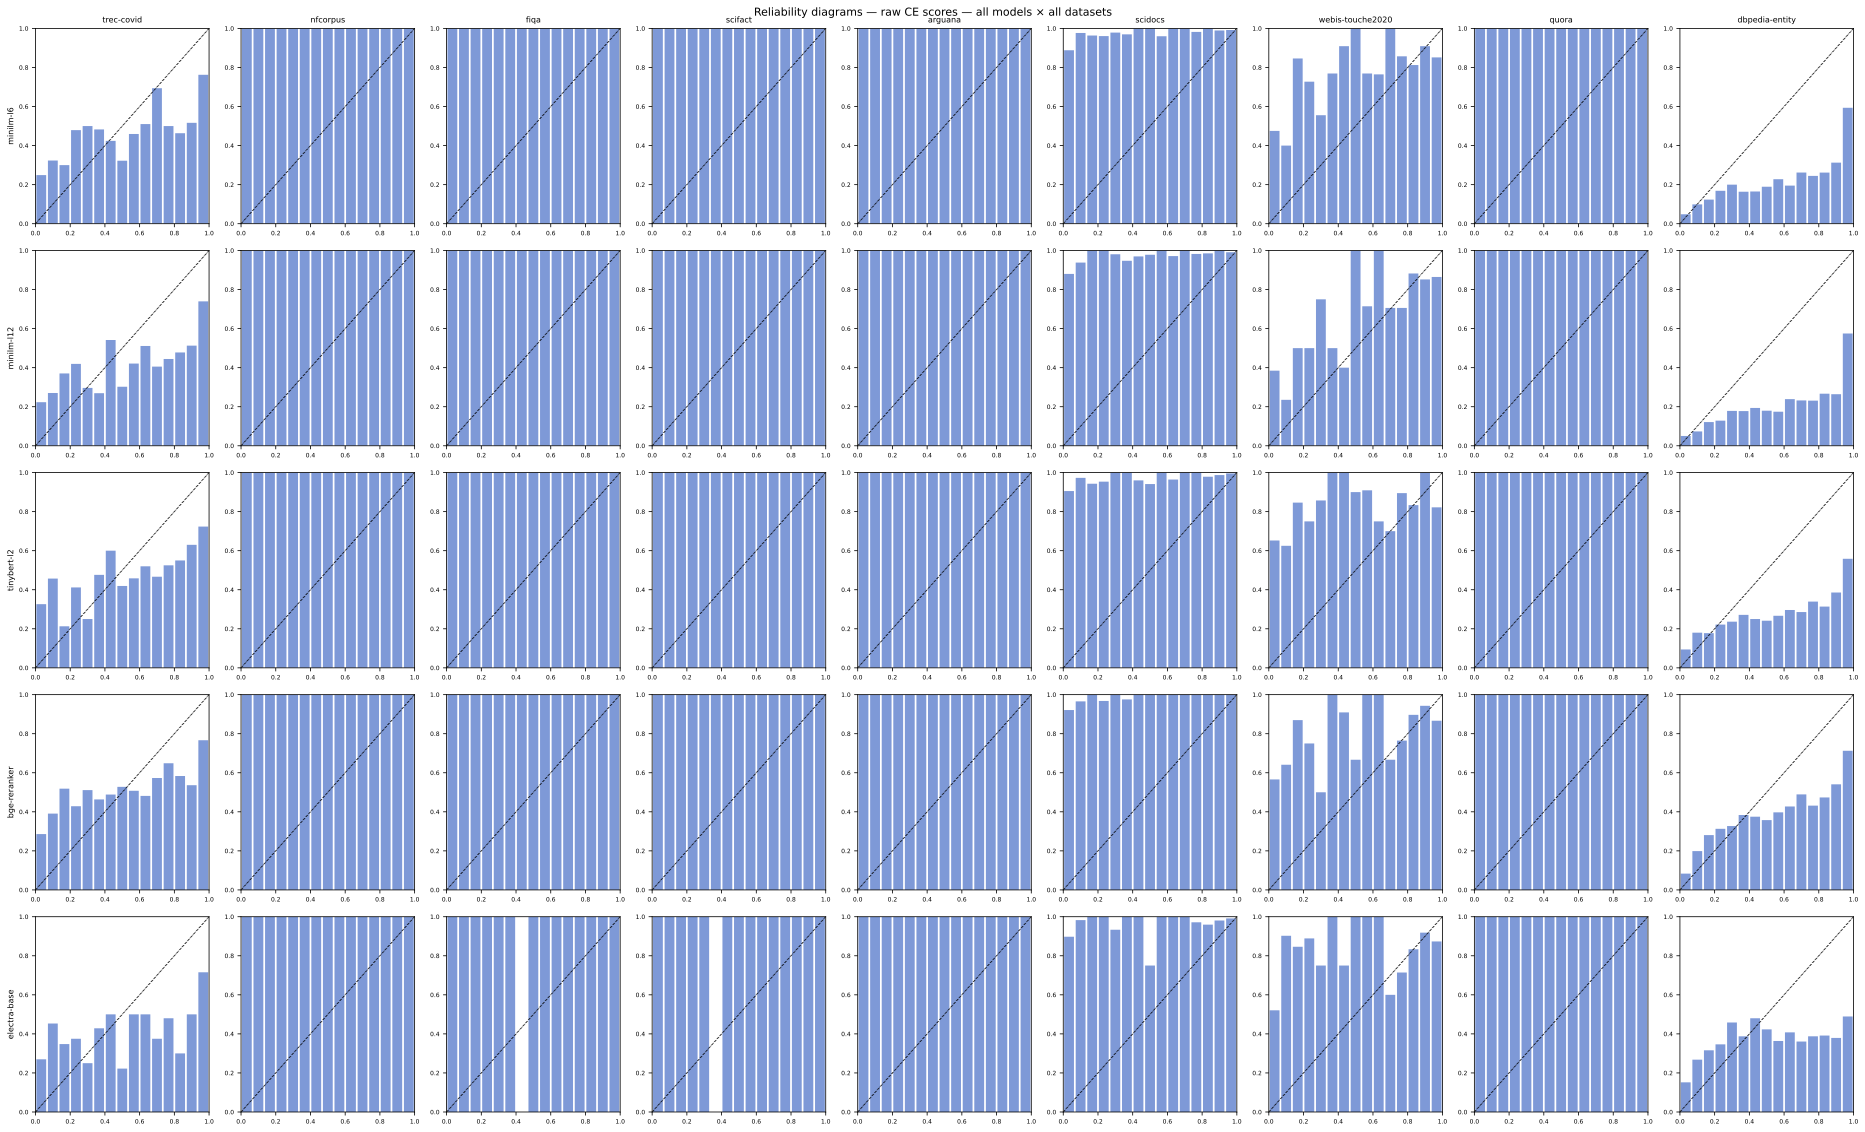
\includegraphics[width=\textwidth]{paper_all_models_all_datasets_raw.png}
\caption{Raw reliability diagrams for all five models (rows) across all nine
datasets (columns). The dashed diagonal denotes perfect calibration; bars below
it indicate overconfidence.}\label{fig:grid}
\end{figure}

\begin{figure}[t]
\centering
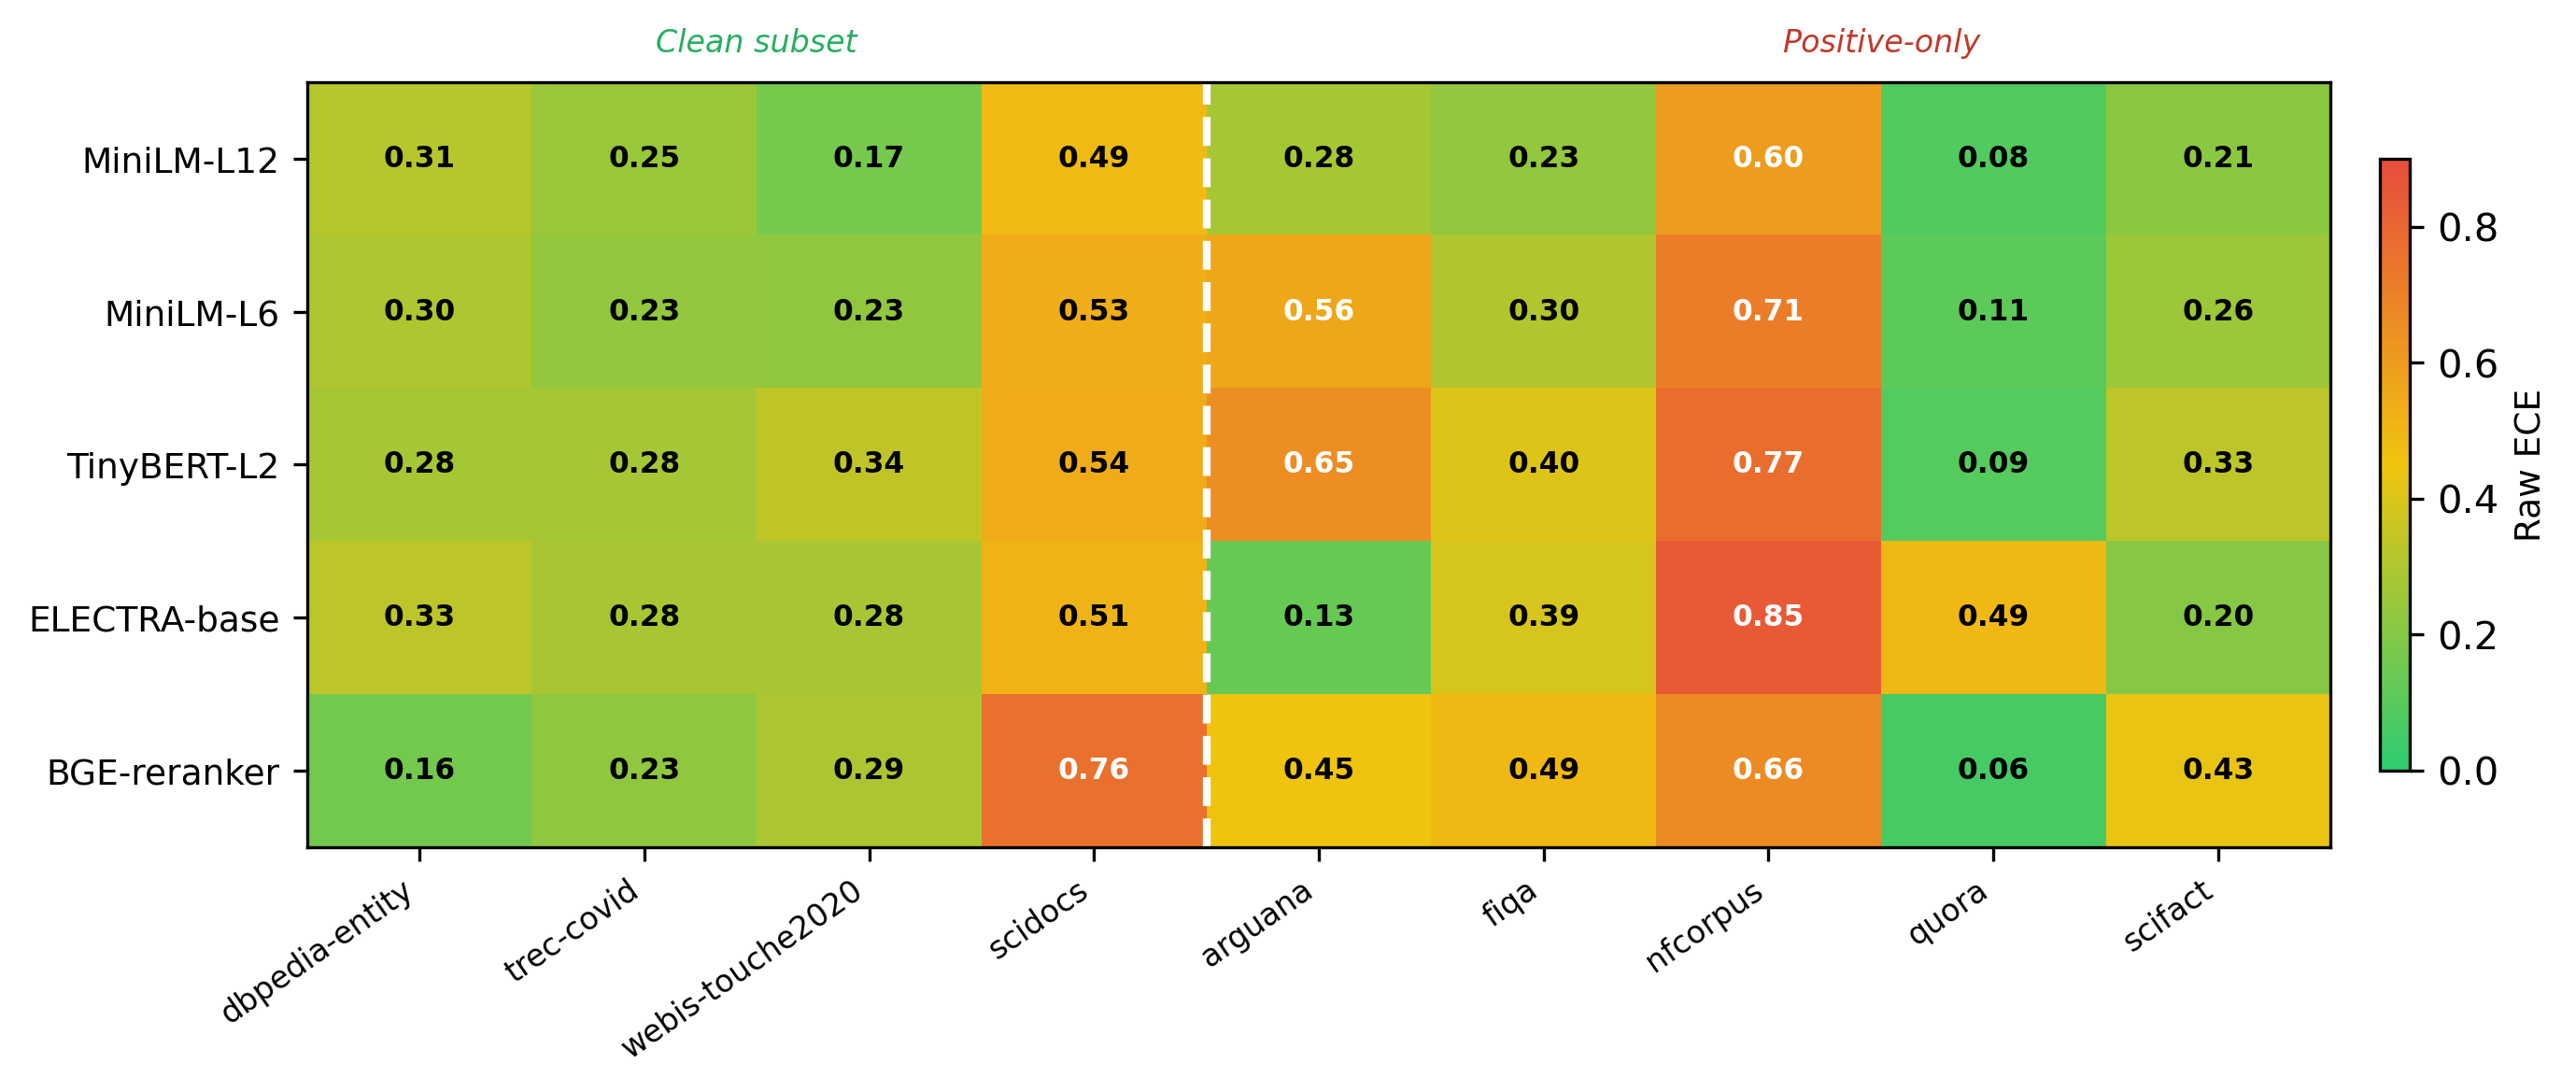
\includegraphics[width=\textwidth]{paper_fig_ece_heatmap.png}
\caption{Raw ECE across all model--dataset pairs. Green denotes low error and red
high error. The dashed line separates the clean subset (left) from the
positive-only datasets (right).}\label{fig:heatmap}
\end{figure}

Table~\ref{tab:raw} quantifies the pattern per dataset. Even trec-covid, the
best-calibrated dataset among the clean four, exhibits a mean ECE of $0.251$ with
a bootstrap interval of $[0.207, 0.299]$. The highest value is $0.716$ on
nfcorpus, a figure that must be interpreted cautiously given its prevalence of
$1.00$. Per-model summaries appear in Table~\ref{tab:permodel}. Mean optimal
temperatures range from $7.3$ for MiniLM-L12 to $12.1$ for TinyBERT; a temperature
near ten implies that the logit must be divided by ten before the sigmoid produces
a value resembling a probability. The most extreme individual case is ELECTRA on
nfcorpus, with a raw ECE of $0.846$.

\begin{table}[t]
\centering
\caption{Raw calibration metrics per dataset (mean over five models), ordered by
prevalence. Bootstrap $95\%$ confidence intervals are query-level with $1{,}000$
resamples. Per-pair intervals are released with the data.}\label{tab:raw}
\small
\begin{tabular}{lrllrr}
\toprule
\rowcolor{headblue}
\thead{Dataset} & \thead{Prev.} & \thead{mean ECE} & \thead{95\% CI} & \thead{mean MCE} & \thead{mean Brier} \\
\midrule
\rowcolor{cleangreen}
dbpedia-entity   & 0.35 & 0.276 & [0.256, 0.297] & 0.527 & 0.290 \\
\rowcolor{cleangreen}
trec-covid       & 0.62 & 0.251 & [0.207, 0.299] & 0.409 & 0.268 \\
\rowcolor{cleangreen}
webis-touche2020 & 0.78 & 0.257 & [0.215, 0.311] & 0.675 & 0.259 \\
\rowcolor{cleangreen}
scidocs          & 0.95 & 0.562 & [0.537, 0.586] & 0.888 & 0.506 \\
\rowcolor{singleclasspink}
arguana          & 1.00 & 0.404 & [0.385, 0.422] & 0.977 & 0.314 \\
\rowcolor{singleclasspink}
fiqa             & 1.00 & 0.377 & [0.343, 0.410] & 0.983 & 0.303 \\
\rowcolor{singleclasspink}
nfcorpus         & 1.00 & 0.716 & [0.675, 0.756] & 0.991 & 0.659 \\
\rowcolor{singleclasspink}
quora            & 1.00 & 0.163 & [0.147, 0.179] & 0.976 & 0.113 \\
\rowcolor{singleclasspink}
scifact          & 1.00 & 0.308 & [0.260, 0.355] & 0.986 & 0.249 \\
\bottomrule
\end{tabular}
\end{table}

\begin{table}[t]
\centering
\caption{Per-model summary, averaged over nine datasets. $T$ denotes the optimal
temperature. Every model requires substantial softening ($T \gg 1$) to align its
scores with empirical accuracy.}\label{tab:permodel}
\small
\begin{tabular}{lrrrr}
\toprule
\rowcolor{headblue}
\thead{Model} & \thead{Params} & \thead{mean $T$} & \thead{mean raw ECE} & \thead{mean iso ECE} \\
\midrule
\rowcolor{rowlight}
MiniLM-L12   & 33M  & 7.34  & 0.292 & 0.013 \\
\rowcolor{rowwhite}
MiniLM-L6    & 22M  & 9.57  & 0.359 & 0.012 \\
\rowcolor{rowlight}
BGE-reranker & 278M & 10.62 & 0.394 & 0.009 \\
\rowcolor{rowwhite}
ELECTRA-base & 110M & 11.60 & 0.386 & 0.012 \\
\rowcolor{rowlight}
TinyBERT-L2  & 4M   & 12.06 & 0.409 & 0.011 \\
\bottomrule
\end{tabular}
\end{table}

The temperature search was capped at twenty. Fifteen of the forty-five
model--dataset pairs reached this ceiling, all of them on single-class or
near-single-class data; for these pairs the reported temperature is a lower bound,
and such values are written $T \geq 20$. Finally, within these five models size does not
predict calibration quality: the Spearman correlation between parameter count and
mean raw ECE is $\rho = -0.10$ ($p = 0.87$). MiniLM-L12, at $33$M parameters,
attains a lower mean ECE than BGE at $278$M. We report this null result here
because it is what a study restricted to one model family and one training corpus
yields, and because Section~\ref{sec:modelscope} shows it does not survive the
addition of models drawn from outside that family. It should therefore be read as
a statement about the homogeneity of this model set rather than about scale.

\subsection{A methodological hazard: positive-only judgments invalidate
calibration evaluation}\label{sec:hazard}
The most consequential finding of this study concerns the five datasets whose
prevalence equals exactly $1.00$. On such data, every judged document is relevant,
and calibration evaluation becomes degenerate. A calibrator that maps all
predicted probabilities toward one attains an ECE near zero, because both the
labels and the predictions concentrate at unity; this reflects the label
distribution, not calibration quality.

Isotonic regression exhibits precisely this behaviour. On single-class fitting
splits it learns to map all inputs to the majority class and, on the held-out
split, reports an ECE of $0.000$. Absent knowledge of its origin, this figure
appears exemplary, but it is an artifact of the evaluation configuration. The harm
extends beyond the isotonic figures to the entire method comparison. Pooling all
forty-five model--dataset pairs and asking how often temperature scaling improves
ECE yields $27$ of $45$ (Wilcoxon $p = 0.024$, Cohen's $d = 0.40$), while isotonic
regression appears to improve all $45$. The naive inference, that temperature
scaling is unreliable and isotonic regression is near-infallible, is incorrect in
both parts.

The mechanism is straightforward. On a single-class fitting split, the temperature
optimiser observes no negative examples, so the negative log-likelihood objective
provides no signal to reduce confidence; the temperature drifts to the ceiling or
moves in the wrong direction. Figure~\ref{fig:backfire} illustrates this on
scifact, where temperature scaling increases ECE while isotonic regression attains
a trivial zero. Neither outcome reflects genuine calibration.

\begin{figure}[t]
\centering
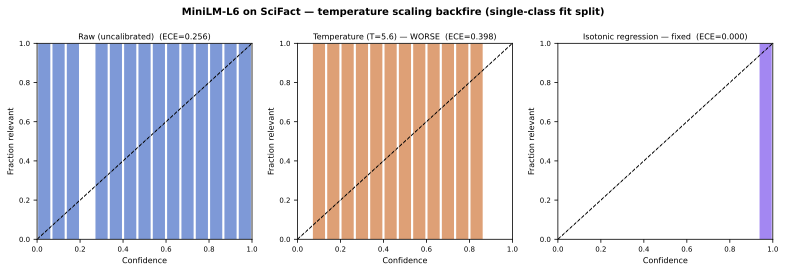
\includegraphics[width=0.85\textwidth]{paper_fig2_minilm_scifact_temp_backfire.png}
\caption{MiniLM-L6 on scifact (prevalence $1.0$). Temperature scaling worsens ECE
while isotonic regression attains a trivial zero. Both outcomes follow from the
absence of negative judgments rather than from the properties of the
methods.}\label{fig:backfire}
\end{figure}

\paragraph{Relation to the incomplete-judgments literature.}
It is natural to ask whether this is the well-known incompleteness problem of
Section~\ref{sec:rw-recent} under another name. It is not, and the distinction is
worth stating precisely because the two are easily conflated.

The established problem concerns \emph{unjudged} documents. Because a run contains
documents the assessors never saw, treating them as non-relevant penalises systems
that retrieve relevant material outside the pool, and ranking metrics computed that
way are biased and unstable \cite{buckley2004,lu2016}. The remedies follow from that
diagnosis: bpref counts only judged documents, inferred measures estimate the
missing mass \cite{yilmaz2006}, and condensed-list evaluation deletes unjudged
documents from the run \cite{sakai2007}.

Three things distinguish the present hazard. First, and decisively, \emph{it
survives the standard remedy}. Condensed-list evaluation is judged-only evaluation,
which is precisely the convention we adopt throughout, and the degeneracy documented
above arises entirely within the judged set. Discarding unjudged documents does not
mitigate the problem; it is the regime in which the problem occurs. Second, the
mechanism differs. The classical concern is missing mass outside the pool, whereas
ours is the class balance inside it: when every judged pair carries the same label,
the quantity ECE estimates is not merely noisy but degenerate, since a constant
predictor attains a perfect score. Third, the consequence differs. Incompleteness
depresses and destabilises the value of a ranking metric, leaving the comparison
between systems approximately intact under the corrected measures; the degeneracy
here \emph{inverts} the comparison between calibration methods, making the trivial
method appear best and a sound method appear unreliable, as the pooled analysis
above demonstrates. A study could apply every remedy in the incompleteness
literature and still reach the wrong conclusion about which calibrator to deploy,
because those remedies repair ranking metrics and are silent about probabilities.

The two problems are therefore complementary rather than competing, and both are
consequences of how test collections are constructed. What the calibration setting
adds is that judgment structure can invalidate a metric outright rather than bias
it, and that the affected collections can be identified in advance.

\smallskip
The appropriate remedy is to restrict method comparisons to datasets on which the
evaluation is well defined, namely those containing a sufficient number of genuine
negative judgments. The next section makes that criterion precise.

\subsection{A pre-flight validity diagnostic}\label{sec:diagnostic}
An observation that a hazard exists is of limited use unless it can be acted upon
before the fact. We therefore state the criterion as an explicit check, fixed in
advance of inspecting any calibration result, that a practitioner can apply to any
collection prior to reporting a calibration figure.

\smallskip
\noindent\textbf{Diagnostic.} Let $n_{+}$ and $n_{-}$ denote the number of judged
positive and negative pairs, and let $\pi = n_{+}/(n_{+}+n_{-})$ be the prevalence.
Calibration evaluation on the collection is treated as \emph{valid} only if
\begin{equation}
\min(n_{+}, n_{-}) \;\geq\; 100
\qquad\text{and}\qquad
\pi \;\leq\; 0.90 .
\label{eq:diagnostic}
\end{equation}
The first condition ensures that the minority class supplies enough support for the
per-bin accuracy estimates that ECE aggregates; the second excludes collections so
skewed that a constant predictor attains a near-zero score. Both thresholds are
conventional rather than tuned, and neither was adjusted after seeing the outcome.

Table~\ref{tab:diagnostic} applies the criterion to all eleven collections used in
this study, comprising the nine BEIR datasets and the two TREC Deep Learning
collections introduced below. Six are flagged. Five are the positive-only BEIR
datasets already identified, for which $n_{-}=0$ and the test fails trivially. The sixth is more informative: scidocs
passes no plausible reading of ``contains genuine negatives'' on inspection, since
it possesses only $91$ judged negatives against $1{,}683$ positives, yet it would
survive a criterion phrased in terms of prevalence alone at any threshold above
$0.95$. Its inclusion in a naive clean subset is therefore a latent error that the
support condition catches.

Two further symptoms, each established elsewhere in this paper without reference to
the diagnostic, confirm that scidocs is degenerate. Its fitted temperature diverges
once the optimiser is permitted to search freely (Section~\ref{sec:robustness}),
behaviour otherwise confined to the positive-only collections. It is also the only
member of the putative clean subset whose cross-domain transfer behaviour departs
from that of its neighbours (Section~\ref{sec:transfer}). A criterion fixed in
advance and two unrelated empirical signatures thus converge on the same
collection, which is the strongest evidence available to us that the criterion
tracks a real property rather than an arbitrary cut.

The diagnostic also motivated an extension of the collection set. Since it is the
scarcity of judged negatives that constrains the study, we added the TREC Deep
Learning 2019 and 2020 passage collections \cite{craswell2020}, which are pooled to
far greater depth than BEIR and consequently supply more negatives than any BEIR
collection used here: $3{,}000$ and $4{,}727$ respectively, at prevalences of
$0.35$ and $0.17$.\footnote{Judgments are graded $0$--$3$; following the collection
convention we treat grade $\geq 2$ as relevant, grade $1$ denoting a passage
related to the query but not answering it. The $\geq 1$ binarisation used for BEIR
is also released, and the conclusions are unchanged under it.} Both pass the
diagnostic comfortably. Protocol differs in one respect: because the official
top-1000 pool file is not rank-ordered and truncation at rank 100 would discard the
majority of the negative judgments that make these collections valuable, we score
every judged pair within the pool rather than a top-100 prefix. Calibration is
measured on judged pairs irrespective of retrieval rank, so this affects the number
of available pairs, not the comparability of the metric.

Accordingly, the primary analyses that follow are conducted on the five collections
that pass Equation~\eqref{eq:diagnostic}: dbpedia-entity, trec-covid,
webis-touche2020, trec-dl-2019, and trec-dl-2020, hereafter the \emph{core subset},
comprising twenty-five model--collection pairs. Results on the four-dataset BEIR
subset that includes scidocs are reported alongside for continuity, and every
qualitative conclusion is unchanged between them. The five positive-only
collections retain value for characterising the pattern of overconfidence but
cannot support conclusions about the relative merits of calibration methods.

\begin{table}[t]
\centering
\caption{The validity diagnostic of Equation~\eqref{eq:diagnostic} applied to all
eleven collections, ordered by prevalence. Six fail. Note scidocs, which is
excluded by the minority-support condition despite a prevalence below the stated
ceiling, and the two TREC Deep Learning collections, whose deep pooling supplies
more negative judgments than any BEIR collection
studied.}\label{tab:diagnostic}
\small
\begin{tabular}{lrrrrc}
\toprule
\rowcolor{headblue}
\thead{Collection} & \thead{$n$ judged} & \thead{$\pi$} & \thead{$n_{-}$} & \thead{$\min(n_+,n_-)$} & \thead{Verdict} \\
\midrule
\rowcolor{cleangreen}
trec-dl-2020     & 5{,}686 & 0.17 & 4{,}727 & 959     & valid \\
\rowcolor{cleangreen}
dbpedia-entity   & 9{,}182 & 0.35 & 5{,}996 & 3{,}186 & valid \\
\rowcolor{cleangreen}
trec-dl-2019     & 4{,}612 & 0.35 & 3{,}000 & 1{,}612 & valid \\
\rowcolor{cleangreen}
trec-covid       & 3{,}475 & 0.62 & 1{,}306 & 1{,}306 & valid \\
\rowcolor{cleangreen}
webis-touche2020 & 635     & 0.78 & 140     & 140     & valid \\
\rowcolor{singleclasspink}
scidocs          & 1{,}774 & 0.95 & 91      & 91      & \textbf{invalid} \\
\rowcolor{singleclasspink}
arguana          & 1{,}316 & 1.00 & 0       & 0       & invalid \\
\rowcolor{singleclasspink}
fiqa             & 756     & 1.00 & 0       & 0       & invalid \\
\rowcolor{singleclasspink}
nfcorpus         & 1{,}941 & 1.00 & 0       & 0       & invalid \\
\rowcolor{singleclasspink}
quora            & 1{,}278 & 1.00 & 0       & 0       & invalid \\
\rowcolor{singleclasspink}
scifact          & 298     & 1.00 & 0       & 0       & invalid \\
\bottomrule
\end{tabular}
\end{table}

\subsection{On data with genuine negatives, all three methods succeed and a
consistent ordering emerges}\label{sec:clean}
On the core subset (five collections, twenty-five model--collection pairs), every
method improves ECE. Temperature scaling reduces mean ECE from $0.280$ to $0.177$,
Platt scaling to $0.046$, and isotonic regression to $0.029$. This directly
contradicts the impression created by the pooled analysis of
Section~\ref{sec:hazard}. The additional intercept parameter available to Platt
scaling permits correction of systematic offsets in the logit distribution that a
scale-only transform cannot address; isotonic regression, being non-parametric,
improves further still. The improvement from temperature to Platt
($0.177 \to 0.046$) exceeds that from Platt to isotonic ($0.046 \to 0.029$), which
bears on the practical trade-off between flexibility and overfitting risk on small
calibration sets.

Table~\ref{tab:core} gives the per-collection breakdown. The ordering isotonic $>$
Platt $>$ temperature holds on every collection, but the margin between temperature
and the two-parameter methods varies sharply with prevalence. On trec-dl-2020
($\pi = 0.17$) temperature achieves only $0.284$ against Platt's $0.021$, whereas
on trec-covid ($\pi = 0.62$) the two are nearly indistinguishable ($0.056$ against
$0.054$). This is the intercept mechanism made visible: the further the class
balance departs from the point at which the sigmoid is centred, the more of the
correction must come from a shift that temperature cannot supply.

The same ordering holds on the four-dataset BEIR subset that includes scidocs,
reported per pair in Table~\ref{tab:clean}, where mean ECE falls from $0.340$ raw
to $0.232$ (temperature), $0.045$ (Platt), and $0.025$ (isotonic), with all twenty
pairs improving under each method.

\begin{table}[t]
\centering
\caption{Mean ECE by collection on the core subset (five models each), ordered by
prevalence. The ordering isotonic $>$ Platt $>$ temperature holds throughout, but
temperature's deficit widens as prevalence departs from balance.}\label{tab:core}
\small
\begin{tabular}{lrrrrr}
\toprule
\rowcolor{headblue}
\thead{Collection} & \thead{$\pi$} & \thead{raw} & \thead{temp.} & \thead{Platt} & \thead{iso.} \\
\midrule
\rowcolor{cleangreen}
trec-dl-2020     & 0.17 & 0.324 & 0.284 & 0.021 & 0.016 \\
\rowcolor{cleangreen}
dbpedia-entity   & 0.35 & 0.276 & 0.182 & 0.030 & 0.022 \\
\rowcolor{cleangreen}
trec-dl-2019     & 0.35 & 0.285 & 0.146 & 0.043 & 0.039 \\
\rowcolor{cleangreen}
trec-covid       & 0.62 & 0.255 & 0.056 & 0.054 & 0.031 \\
\rowcolor{cleangreen}
webis-touche2020 & 0.78 & 0.262 & 0.221 & 0.082 & 0.038 \\
\midrule
\rowcolor{bestcell}
\textbf{Mean}    &      & \textbf{0.280} & \textbf{0.177} & \textbf{0.046} & \textbf{0.029} \\
\bottomrule
\end{tabular}
\end{table}

Because six comparisons are drawn from the same data, we apply Holm--Bonferroni
correction across the full family rather than reporting each in isolation.
Table~\ref{tab:stats} reports the outcome: all six survive at $\alpha = 0.05$, the
largest adjusted $p$-value being $1.05\times10^{-4}$. A per-dataset breakdown is
also more informative than a single pooled test, and it is uniform: on each of the
four datasets individually, every method beats the raw baseline in all five models.

\begin{table}[t]
\centering
\caption{Method comparisons with Holm--Bonferroni correction across the family of
six tests (clean subset, $n=20$ pairs). Negative $\Delta$ favours the first-named
method. All six survive correction.}\label{tab:stats}
\small
\begin{tabular}{lrrrrc}
\toprule
\rowcolor{headblue}
\thead{Comparison} & \thead{mean $\Delta$} & \thead{$d_z$} & \thead{wins} & \thead{$p_{\text{Holm}}$} & \thead{Sig.} \\
\midrule
\rowcolor{rowlight}
temperature vs.\ raw   & $-0.108$ & $-1.37$ & 20/20 & $1.1\times10^{-5}$ & yes \\
\rowcolor{rowwhite}
Platt vs.\ raw         & $-0.295$ & $-1.72$ & 20/20 & $1.1\times10^{-5}$ & yes \\
\rowcolor{rowlight}
isotonic vs.\ raw      & $-0.314$ & $-1.97$ & 20/20 & $1.1\times10^{-5}$ & yes \\
\rowcolor{rowwhite}
Platt vs.\ temperature & $-0.187$ & $-1.08$ & 17/20 & $9.5\times10^{-5}$ & yes \\
\rowcolor{rowlight}
isotonic vs.\ temperature & $-0.206$ & $-1.26$ & 20/20 & $1.1\times10^{-5}$ & yes \\
\rowcolor{rowwhite}
isotonic vs.\ Platt    & $-0.019$ & $-0.86$ & 18/20 & $1.1\times10^{-4}$ & yes \\
\bottomrule
\end{tabular}
\end{table}

Figure~\ref{fig:fixworks} depicts the progression on a representative clean
example, BGE-reranker on trec-covid: the raw bars lie well below the diagonal,
temperature scaling raises them partway, and Platt and isotonic bring them close
to the diagonal. Figure~\ref{fig:cleangrid} confirms the pattern across all models
and clean datasets.

\begin{table}[t]
\centering
\caption{Full results on the clean subset (four datasets with genuine negatives),
held-out split. All three methods reduce error in every pair, in the consistent
order isotonic $>$ Platt $>$ temperature.}\label{tab:clean}
\scriptsize
\setlength{\tabcolsep}{3.5pt}
\begin{tabular}{llrrrrrrr}
\toprule
\rowcolor{headblue}
\thead{Model} & \thead{Dataset} & \thead{Prev.} & \thead{raw ECE} & \thead{$T$} & \thead{temp ECE} & \thead{Platt ECE} & \thead{iso ECE} & \thead{$\Delta_{\text{iso}}$} \\
\midrule
\rowcolor{rowlight}
MiniLM-L6   & dbpedia-entity   & 0.35 & 0.297 & 5.83  & 0.219 & 0.027 & 0.024 & $-0.273$ \\
\rowcolor{rowwhite}
MiniLM-L6   & trec-covid       & 0.62 & 0.235 & 4.40  & 0.045 & 0.044 & 0.027 & $-0.208$ \\
\rowcolor{rowlight}
MiniLM-L6   & webis-touche2020 & 0.78 & 0.229 & 4.83  & 0.215 & 0.103 & 0.050 & $-0.179$ \\
\rowcolor{rowwhite}
MiniLM-L6   & scidocs          & 0.95 & 0.534 & $\geq$20 & 0.465 & 0.018 & 0.011 & $-0.523$ \\
\rowcolor{rowlight}
MiniLM-L12  & dbpedia-entity   & 0.35 & 0.313 & 6.59  & 0.221 & 0.028 & 0.019 & $-0.295$ \\
\rowcolor{rowwhite}
MiniLM-L12  & trec-covid       & 0.62 & 0.251 & 4.84  & 0.058 & 0.044 & 0.042 & $-0.209$ \\
\rowcolor{rowlight}
MiniLM-L12  & webis-touche2020 & 0.78 & 0.166 & 3.97  & 0.160 & 0.110 & 0.038 & $-0.129$ \\
\rowcolor{rowwhite}
MiniLM-L12  & scidocs          & 0.95 & 0.488 & $\geq$20 & 0.458 & 0.017 & 0.015 & $-0.472$ \\
\rowcolor{rowlight}
TinyBERT-L2 & dbpedia-entity   & 0.35 & 0.281 & 6.75  & 0.196 & 0.030 & 0.025 & $-0.256$ \\
\rowcolor{rowwhite}
TinyBERT-L2 & trec-covid       & 0.62 & 0.276 & 6.48  & 0.055 & 0.057 & 0.033 & $-0.243$ \\
\rowcolor{rowlight}
TinyBERT-L2 & webis-touche2020 & 0.78 & 0.339 & 11.08 & 0.244 & 0.060 & 0.032 & $-0.307$ \\
\rowcolor{rowwhite}
TinyBERT-L2 & scidocs          & 0.95 & 0.540 & $\geq$20 & 0.467 & 0.004 & 0.009 & $-0.532$ \\
\rowcolor{rowlight}
BGE-reranker& dbpedia-entity   & 0.35 & 0.159 & 2.96  & 0.107 & 0.028 & 0.022 & $-0.137$ \\
\rowcolor{rowwhite}
BGE-reranker& trec-covid       & 0.62 & 0.228 & 4.39  & 0.037 & 0.041 & 0.028 & $-0.199$ \\
\rowcolor{rowlight}
BGE-reranker& webis-touche2020 & 0.78 & 0.292 & 6.78  & 0.236 & 0.068 & 0.019 & $-0.274$ \\
\rowcolor{rowwhite}
BGE-reranker& scidocs          & 0.95 & 0.762 & $\geq$20 & 0.488 & 0.006 & 0.012 & $-0.751$ \\
\rowcolor{rowlight}
ELECTRA-base& dbpedia-entity   & 0.35 & 0.330 & 6.84  & 0.164 & 0.035 & 0.021 & $-0.309$ \\
\rowcolor{rowwhite}
ELECTRA-base& trec-covid       & 0.62 & 0.285 & 4.77  & 0.084 & 0.084 & 0.025 & $-0.260$ \\
\rowcolor{rowlight}
ELECTRA-base& webis-touche2020 & 0.78 & 0.283 & 6.10  & 0.249 & 0.068 & 0.052 & $-0.231$ \\
\rowcolor{rowwhite}
ELECTRA-base& scidocs          & 0.95 & 0.512 & $\geq$20 & 0.466 & 0.019 & 0.008 & $-0.504$ \\
\midrule
\rowcolor{cleangreen}
\multicolumn{3}{l}{\textbf{Mean (clean)}} & \textbf{0.340} & & \textbf{0.232} & \textbf{0.045} & \textbf{0.025} & \\
\bottomrule
\end{tabular}
\end{table}

\begin{figure}[t]
\centering
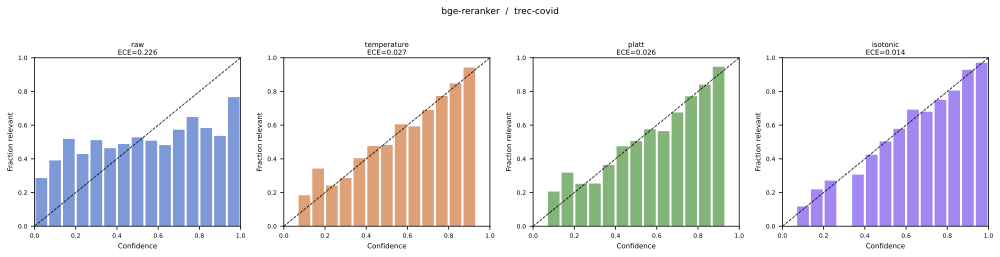
\includegraphics[width=0.95\textwidth]{paper_fig_bge_treccovid_4panel.png}
\caption{BGE-reranker on trec-covid (prevalence $0.62$): raw, temperature, Platt,
and isotonic calibration. Because this dataset contains genuine negatives, the ECE
reductions are meaningful.}\label{fig:fixworks}
\end{figure}

\begin{figure}[t]
\centering
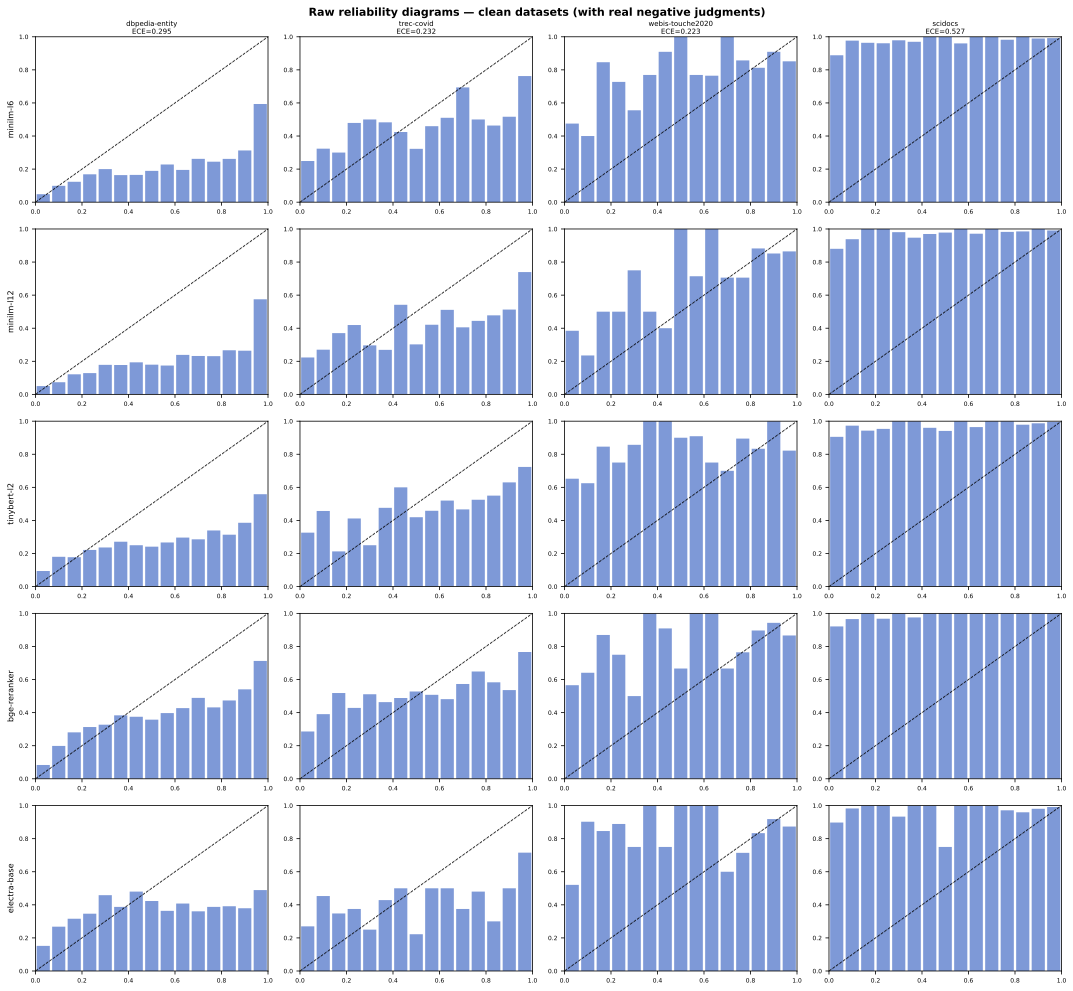
\includegraphics[width=\textwidth]{paper_fig3_all_models_clean_datasets.png}
\caption{Raw reliability diagrams on the clean subset: five models by four
datasets with genuine negatives. The consistent gap below the diagonal indicates
overconfidence on data where the measurement is well
defined.}\label{fig:cleangrid}
\end{figure}

\subsection{Model scope: newer and larger re-rankers are better calibrated, but
not because they are larger}\label{sec:modelscope}
The five models considered so far top out at $278$M parameters and were all
fine-tuned on MS~MARCO, which limits what can be concluded about calibration as a
function of scale or training data. We therefore added two further re-rankers
selected to break both constraints: BGE-reranker-large ($560$M), which doubles the
largest parameter count, and mxbai-rerank-base ($184$M), a DeBERTa-v3 model trained
without MS~MARCO supervision. Both were scored on exactly the pair sets used for the
original models, so the comparison is like for like.

Table~\ref{tab:modelscope} reports the outcome on the core subset. The two added
models are markedly better calibrated before any correction: mean raw ECE of $0.169$
against $0.280$ for the original five. They also require far gentler correction,
with median optimal temperatures near $2$--$3$ against $6$--$8$. On the face of it
this is a scale effect, and the correlation between parameter count and raw ECE,
which was statistically indistinguishable from zero across the original five models
($\rho = -0.10$, $p = 0.87$), becomes strong and significant across all seven
($\rho = -0.86$, $p = 0.01$).

We do not think that correlation should be read as an effect of scale, and we report
it with the confound stated rather than as a finding about size. The decisive
observation is internal to the extension: mxbai-rerank-base, at $184$M parameters,
is the best-calibrated model in the entire study (raw ECE $0.136$), outperforming
BGE-large at three times its size ($0.202$) and BGE-base at $278$M ($0.230$). Size
therefore does not order the models even within the extension. What the two added
models share is not scale but recency of training recipe, and because recipe and
scale move together across the seven models the two cannot be separated by this
design. The honest conclusion is narrower than the correlation suggests: the earlier
null result was an artifact of a narrow and homogeneous model set, calibration
quality does vary substantially with the choice of re-ranker, and identifying which
property is responsible would require models matched on everything but size.

One further observation matters more for practice than either. After Platt scaling
or isotonic regression the seven models converge to within $0.014$ of one another
($0.038$--$0.052$ and $0.025$--$0.036$ respectively), despite spanning a raw range of
$0.136$ to $0.323$. Choosing a better-calibrated re-ranker and calibrating a worse
one are close to substitutable, and the latter is available without changing the
model.

\begin{table}[t]
\centering
\caption{Model-scope extension, core subset (five collections each).
\textcolor{green!50!black}{Green} rows are the added models. The added models are
better calibrated raw and need gentler temperatures, but after Platt or isotonic
correction all seven converge.}\label{tab:modelscope}
\small
\begin{tabular}{lrlrrrrr}
\toprule
\rowcolor{headblue}
\thead{Model} & \thead{Params} & \thead{Training} & \thead{raw} & \thead{$T$} & \thead{temp.} & \thead{Platt} & \thead{iso.} \\
\midrule
\rowcolor{rowlight}
TinyBERT-L2  &    4M & MS MARCO     & 0.323 & 8.69 & 0.202 & 0.044 & 0.030 \\
\rowcolor{rowwhite}
MiniLM-L6    &   22M & MS MARCO     & 0.295 & 6.24 & 0.202 & 0.048 & 0.030 \\
\rowcolor{rowlight}
MiniLM-L12   &   33M & MS MARCO     & 0.296 & 6.84 & 0.197 & 0.052 & 0.029 \\
\rowcolor{rowwhite}
ELECTRA-base &  110M & MS MARCO     & 0.257 & 5.29 & 0.124 & 0.048 & 0.030 \\
\rowcolor{cleangreen}
mxbai-base   &  184M & non-MS MARCO & \textbf{0.136} & 1.99 & 0.123 & 0.043 & 0.033 \\
\rowcolor{rowlight}
BGE-base     &  278M & MS MARCO     & 0.230 & 4.16 & 0.162 & 0.038 & 0.025 \\
\rowcolor{cleangreen}
BGE-large    &  560M & contrastive  & 0.202 & 3.49 & 0.120 & 0.043 & 0.036 \\
\midrule
\rowcolor{rowwhite}
\multicolumn{3}{l}{\textit{Original five (mean)}}   & 0.280 & 6.24 & 0.177 & 0.046 & 0.029 \\
\rowcolor{bestcell}
\multicolumn{3}{l}{\textit{Extension two (mean)}}   & \textbf{0.169} & 2.74 & \textbf{0.122} & 0.043 & 0.035 \\
\bottomrule
\end{tabular}
\end{table}

\subsection{The in-domain method ordering does not survive domain transfer}\label{sec:transfer}
The comparison above assumes a calibration set drawn from the target domain. That
assumption is often unavailable: a practitioner deploying a re-ranker on a new
corpus typically has no labelled relevance judgments for it. The operative question
is therefore whether a calibrator fitted elsewhere can be reused.

To answer it we evaluate three regimes, all on the target domain's held-out split:
an \emph{in-domain} calibrator fitted on the target's own fit split, which serves
as an upper bound; a \emph{transferred} calibrator fitted on the pooled fit splits
of the remaining core domains (leave-one-domain-out); and the uncalibrated
baseline. No new inference is required, since the same stored logits support all
three.

The result, shown in Fig.~\ref{fig:transfer} and Table~\ref{tab:transfer},
substantially qualifies the recommendation of Section~\ref{sec:clean}. Temperature
scaling transfers robustly: the transferred calibrator attains a mean ECE of
$0.191$ against an in-domain bound of $0.177$ and a raw baseline of $0.280$,
retaining $87\%$ of the available benefit and improving on the raw scores in $22$
of $25$ cases. Platt scaling transfers considerably less well, retaining $44\%$ of
its benefit as its mean ECE rises from $0.046$ in-domain to $0.178$. It is also
markedly less reliable: the standard deviation of its transferred error is $0.122$
against temperature's $0.090$, and it is \emph{worse than applying no calibration
at all} in $6$ of $25$ cases, five of which are webis-touche2020, where it fails for
every model.

The contrast is therefore not that Platt scaling is useless out of domain, but that
its advantage is contingent on the target resembling the sources, whereas
temperature's is not. We note that this qualification is itself sensitive to how
many source domains are pooled: with only two sources available, Platt's retention
falls to $8\%$, whereas pooling four sources recovers it to $44\%$. Practitioners
with several labelled domains may therefore transfer Platt with more confidence than
those with one, though temperature remains the safer default in either case.

The mechanism is the same intercept that makes Platt scaling effective in the first
place. An intercept encodes where the decision boundary sits in logit space, and
that location is a property of the domain rather than of the model; transplanting it
imports a bias that pooling can average down but not eliminate. A temperature, by
contrast, encodes the sharpness of the logit distribution, which is comparatively
stable across domains. The fitted temperatures bear this out: across the core subset
the ratio of largest to smallest optimum per model lies between $1.71$ and $2.94$, a
spread narrow enough to justify quoting a single per-model temperature as a
deployment default (Table~\ref{tab:recipe}).

\begin{figure}[t]
\centering
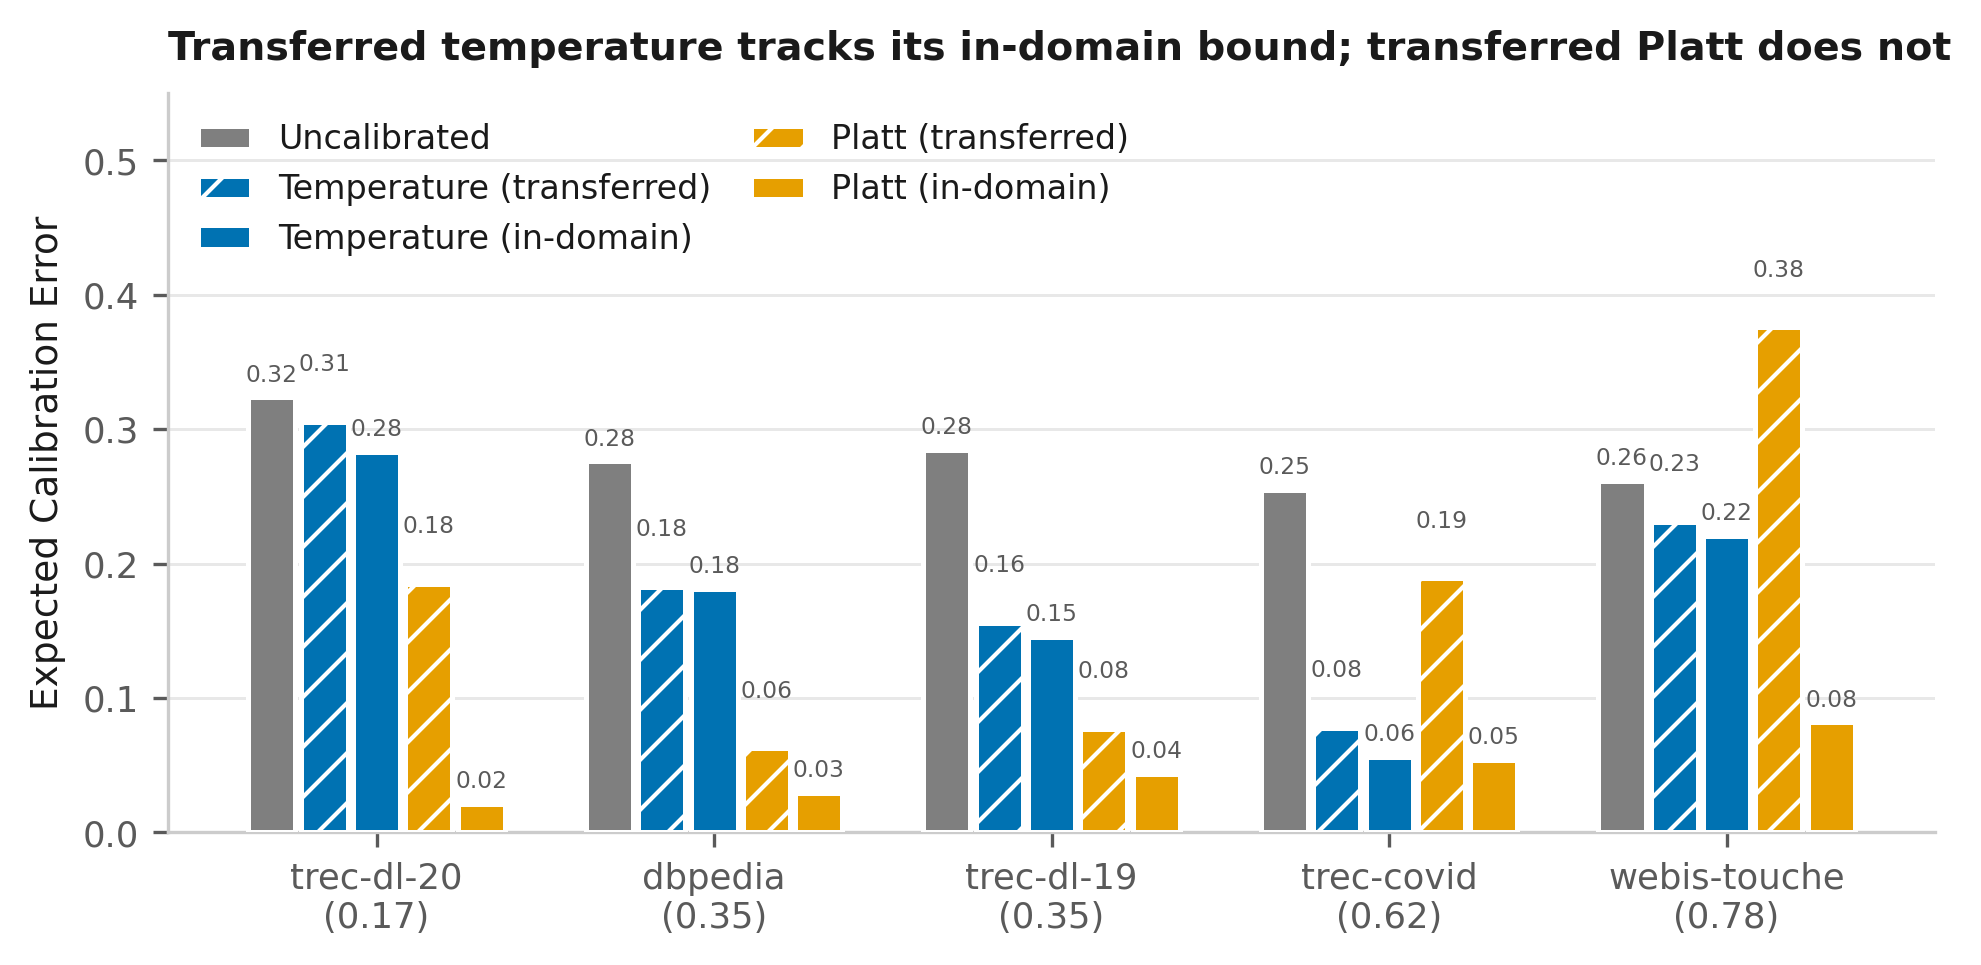
\includegraphics[width=\textwidth]{paper_fig_transfer.png}
\caption{Cross-domain calibrator transfer on the core subset, averaged over five
models. Hatched bars denote calibrators fitted on other domains
(leave-one-domain-out); solid bars denote in-domain fits. Temperature is nearly
unaffected by transfer, whereas Platt scaling degrades to at or above the
uncalibrated baseline.}\label{fig:transfer}
\end{figure}

\begin{table}[t]
\centering
\caption{Calibrator transfer on the core subset ($n=25$ model--collection pairs).
Retention is the fraction of the in-domain ECE reduction that survives transfer.
Temperature retains most of its benefit and is the more stable of the two; Platt
retains less and fails outright on six pairs.}
\label{tab:transfer}
\small
\begin{tabular}{lrrrr}
\toprule
\rowcolor{headblue}
\thead{Regime} & \thead{Temp.\ ECE} & \thead{Platt ECE} & \thead{Temp.\ retention} & \thead{Platt retention} \\
\midrule
\rowcolor{rowlight}
Uncalibrated        & \multicolumn{2}{c}{0.280} & --- & --- \\
\rowcolor{rowwhite}
Transferred (LODO)  & 0.191 & 0.178 & $87\%$ & $44\%$ \\
\rowcolor{rowlight}
In-domain (bound)   & 0.177 & 0.046 & $100\%$ & $100\%$ \\
\midrule
\rowcolor{rowwhite}
Std.\ dev.\ (LODO)  & 0.090 & 0.122 & \multicolumn{2}{l}{\footnotesize lower is more reliable} \\
\midrule
\rowcolor{cleangreen}
\multicolumn{5}{l}{\textbf{Improves on raw:} temperature $22/25$; Platt $19/25$ (all 5 failures on webis-touche2020)} \\
\bottomrule
\end{tabular}
\end{table}

\subsection{What calibration does and does not buy
downstream}\label{sec:downstream}
Because all three post-hoc methods are monotone, they cannot reorder documents.
Table~\ref{tab:downstream} confirms this empirically: the maximum absolute change
in nDCG@10 across all forty-five pairs is $1.0 \times 10^{-4}$. Calibration is
therefore obtained at no cost to ranking effectiveness.

Monotonicity carries a second and less frequently noted consequence. If the induced
order is unchanged, then at any fixed \emph{coverage}, meaning any fixed number of
accepted items, the accepted set is identical before and after calibration, and so
is its precision. The precision--coverage frontier is therefore invariant under
monotone calibration: no such method can improve the achievable trade-off between
how much a system accepts and how often it is right. Stating this plainly
circumscribes what calibration is for. Its value is not that it makes a selective
prediction system better, but that it makes the system's stated confidence mean what
it says, and thereby turns the threshold into a usable control.

That distinction is measurable. Consider an operator who sets a threshold of
$\tau=0.8$, intending to forward only passages believed at least $80\%$ likely to be
relevant. Fig.~\ref{fig:honesty} reports the precision actually realised.
Uncalibrated, it ranges from $0.36$ on trec-dl-2020 to $0.85$ on webis-touche2020, a
spread of $0.497$ centred at $0.603$, well short of the $0.80$ requested. The same
nominal setting therefore denotes five materially different operating points, and
none of them is the one requested; on the worst collection the operator receives less
than half the precision asked for. After isotonic calibration the realised precision
lies between $0.79$ and $0.87$, a spread of $0.078$ and a mean of $0.833$. Platt
scaling gives a spread of $0.106$ and temperature $0.243$. The threshold becomes
portable across collections, which is precisely the property a deployment needs from
it.

Panel~(a) of Fig.~\ref{fig:honesty} shows why the uncalibrated case fails as a
control rather than merely as an estimate. Raising $\tau$ from $0.5$ to $0.8$ moves
the realised precision of the raw scores from $0.685$ to $0.703$, a change of under
two points, because the scores are so compressed toward unity that the threshold
selects almost the same set throughout. The dial is connected to nothing. After
calibration the same sweep moves the operating point substantially.

Two caveats belong with this result. Calibrated scores in our data are mildly
conservative at $\tau = 0.8$, realising $0.85$ against a requested $0.80$, so they
under-promise rather than over-promise; this is the preferable direction of error
but it is not exact. And because calibration redistributes probability mass
downward, a fixed threshold accepts far fewer items after correction, so coverage
falls; thresholds carried over unchanged from an uncalibrated system will need to be
re-tuned. Thresholds above $0.8$ are not reported because too few items clear them
for the realised precision to be estimated reliably.

\begin{figure}[t]
\centering
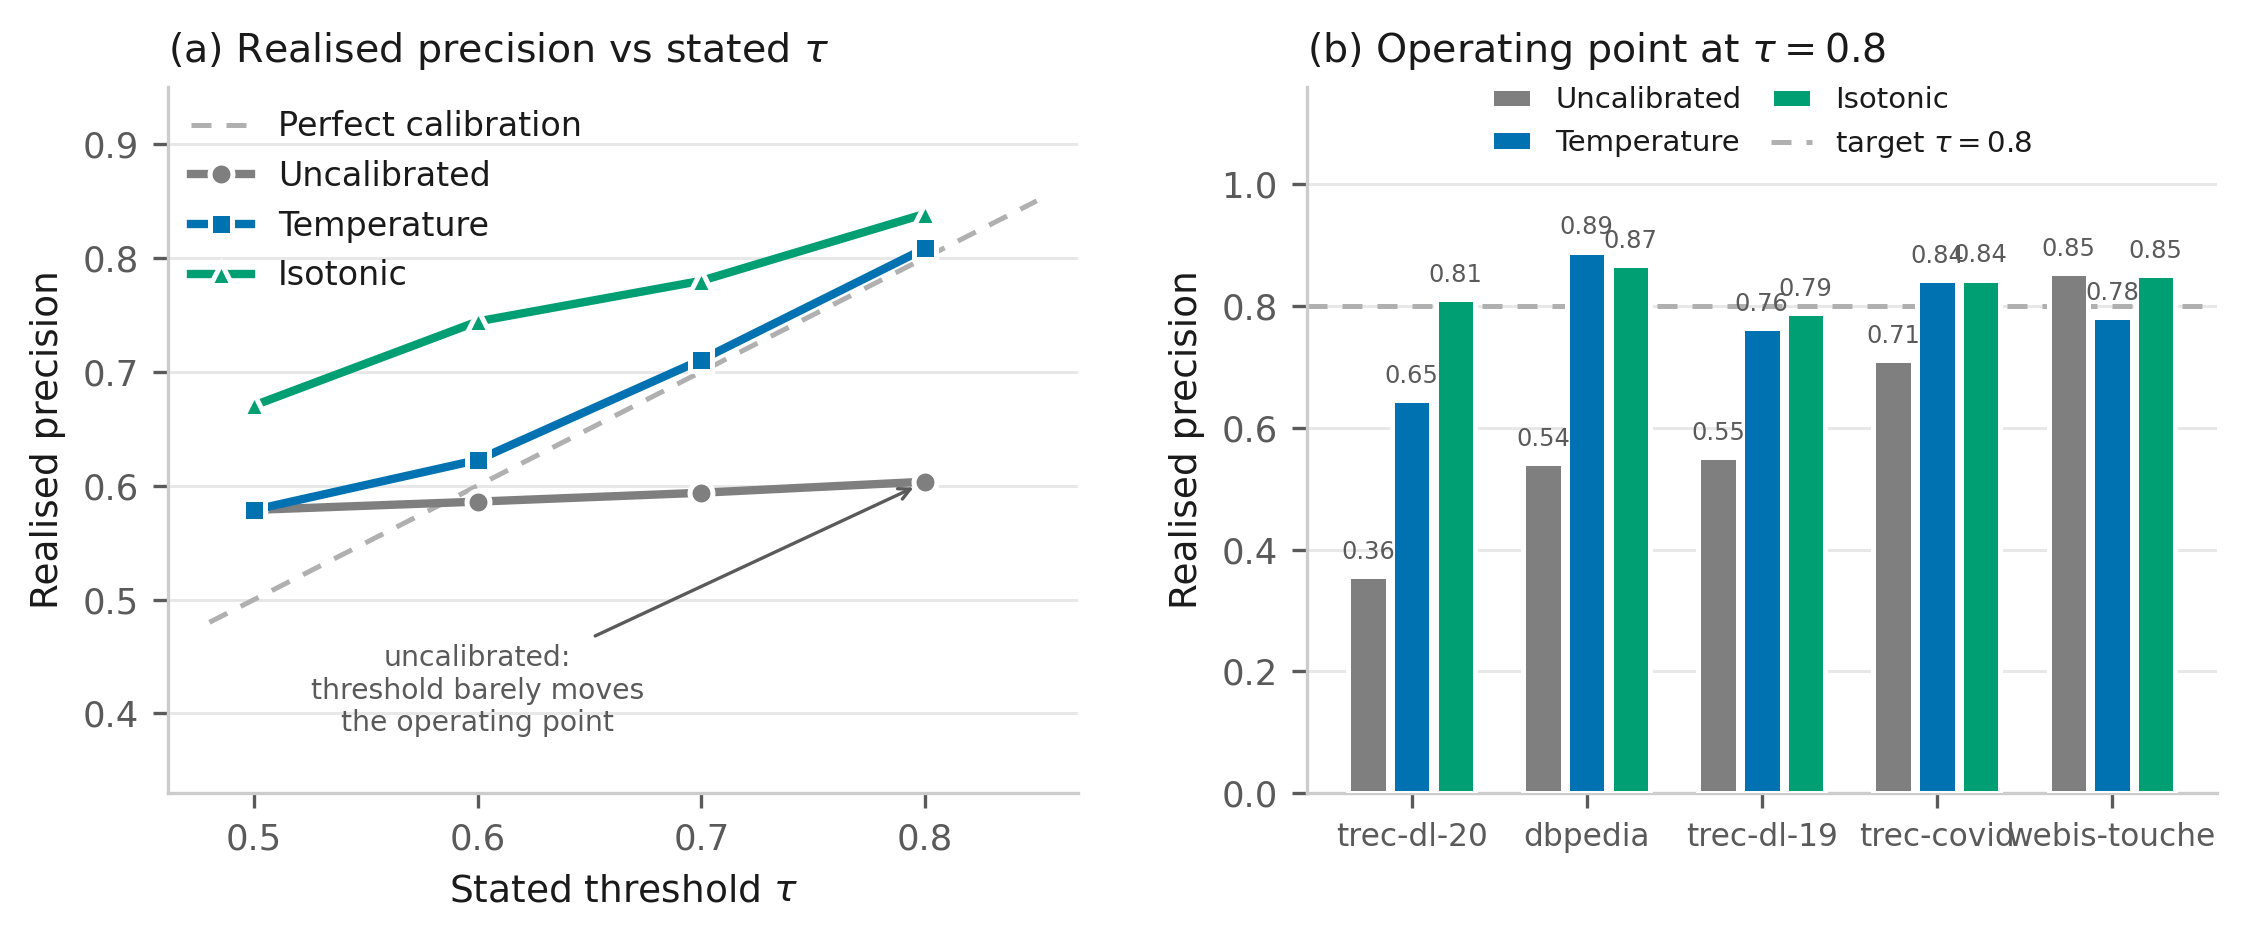
\includegraphics[width=\textwidth]{paper_fig_threshold_honesty.png}
\caption{The operational consequence of miscalibration, core subset, averaged over
five models. (a) Realised precision against the stated threshold $\tau$; the raw
scores are nearly flat, so the threshold barely moves the operating point. (b) At
$\tau=0.8$ the uncalibrated realised precision varies from $0.54$ to $0.85$ across
domains, whereas after calibration the same setting denotes nearly the same
operating point everywhere.}\label{fig:honesty}
\end{figure}

\begin{table}[t]
\centering
\caption{Downstream ranking metrics per dataset (mean over five models). nDCG@10
and MAP are unchanged after calibration. The accept rate at $p > 0.5$ is also
unchanged, because even after division by $T \approx 10$, most scores remain above
$0.5$.}\label{tab:downstream}
\small
\begin{tabular}{lrrrr}
\toprule
\rowcolor{headblue}
\thead{Dataset} & \thead{nDCG@10} & \thead{MAP} & \thead{Accept (raw)} & \thead{Accept (cal)} \\
\midrule
\rowcolor{cleangreen}
dbpedia-entity   & 0.349 & 0.455 & 0.963 & 0.963 \\
\rowcolor{cleangreen}
trec-covid       & 0.686 & 0.680 & 0.988 & 0.988 \\
\rowcolor{cleangreen}
webis-touche2020 & 0.265 & 0.287 & 0.988 & 0.988 \\
\rowcolor{cleangreen}
scidocs          & 0.157 & 0.214 & 0.797 & 0.797 \\
\rowcolor{singleclasspink}
arguana          & 0.253 & 0.181 & 1.000 & 1.000 \\
\rowcolor{singleclasspink}
fiqa             & 0.316 & 0.352 & 0.827 & 0.827 \\
\rowcolor{singleclasspink}
nfcorpus         & 0.315 & 0.389 & 0.599 & 0.599 \\
\rowcolor{singleclasspink}
quora            & 0.780 & 0.751 & 0.922 & 0.922 \\
\rowcolor{singleclasspink}
scifact          & 0.676 & 0.644 & 0.805 & 0.805 \\
\bottomrule
\end{tabular}
\end{table}

The accept rate reported in Table~\ref{tab:downstream} is a special case of the
same phenomenon. At the particular threshold $p>0.5$ it is unchanged after
temperature scaling in all forty-five pairs, because the models are overconfident
by enough that dividing the logit by ten still leaves most scores above one half.
That coincidence at a single threshold should not be read as calibration having no
downstream effect; as the sweep above shows, the effect is substantial once the
threshold is varied, and it is a change in what the threshold \emph{means} rather
than in what the ranking can achieve.

\subsection{Sensitivity to the treatment of unjudged
documents}\label{sec:sensitivity}
Restriction to judged pairs is the standard convention, but in deployment unjudged
documents are nonetheless presented to downstream consumers. To assess the
robustness of the findings, ECE was recomputed under an alternative convention
that treats every unjudged pair as non-relevant. The mean ECE shifts by $-0.167$
across the forty-five pairs, but the direction is inconsistent: error decreases in
$28$ pairs and increases in $17$. The direction is governed by dataset structure.
On positive-only datasets, the influx of pseudo-negative unjudged pairs dilutes
the positive mass and improves the apparent calibration; on datasets that already
contain genuine negatives, the additional pseudo-negatives degrade it. This
reinforces the central methodological point: no assumption-free calibration figure
exists for BEIR, because the judgment structure shapes the metric and must be
reported alongside any ECE value. The judged-only convention is adopted as
primary, and the clean-subset conclusions hold under both treatments.

\subsection{Robustness of the measurement
instrument}\label{sec:robustness}
Two properties of the measurement procedure could in principle drive the reported
results rather than the models. Both are tested here.

\paragraph{Binning.}
ECE is a binned estimator, and its value depends on the binning scheme
\cite{nixon2019,roelofs2022}. We recomputed every ECE under ten schemes: equal-width
and equal-mass (quantile) binning, each at $5$, $10$, $15$, $20$, and $30$ bins. The
mean ECE across all forty-five pairs varies only between $0.3656$ and $0.3690$, and
across the clean subset between $0.3308$ and $0.3385$. At the level of individual
model--dataset pairs, the mean spread between the largest and smallest of the ten
estimates is $0.0039$, with a maximum of $0.0351$. The ranking of models by mean ECE
on the clean subset is identical under nine of the ten schemes, the single exception
transposing the two adjacent middle positions under equal-mass binning at twenty
bins. The conclusions are therefore not an artifact of the binning choice, and the
fixed scheme of fifteen equal-width bins used throughout is representative.

\paragraph{Temperature search bounds.}
The optimiser was bounded at $T \leq 20$, which saturated in fifteen of forty-five
pairs. Refitting with the bound relaxed to $T \leq 1000$ shows that the censoring is
concentrated where the hazard applies: of the fifteen affected pairs, the median
unconstrained optimum is at the new bound itself, indicating genuine divergence
rather than a finite optimum beyond the original ceiling. This is the expected
behaviour on positive-only data. When the labels are uniformly positive but many
logits are negative, the likelihood is improved without limit by driving $T$ upward,
which collapses every probability toward $0.5$; divergence is thus a signature of
the degeneracy rather than a property of the model. On the clean subset only five
pairs are affected, four of them scidocs, and relaxing the bound changes the mean
ECE by $-0.005$. The substantive conclusions are unaffected, and reported
temperatures for censored pairs are retained as $T \geq 20$ to make the censoring
visible.

% =============================================================================
\section{Discussion}\label{sec:discussion}

\paragraph{A deployment recipe.}
For practitioners consuming re-ranker sigmoid outputs as probabilities, the
practical recommendation is that these values should not be used without
correction. Table~\ref{tab:recipe} provides a concrete recipe: for each model, the
mean optimal temperature on the clean subset is reported, and dividing the logit by
this temperature before the sigmoid constitutes a single-line modification that
requires no retraining and substantially improves calibration. Where a held-out
calibration set containing genuine negatives is available, Platt scaling or
isotonic regression will improve upon these temperatures, which should be regarded
as a floor rather than a ceiling.

\begin{table}[t]
\centering
\caption{Deployment recipe: recommended temperature per model, computed as the
mean optimal $T$ on the clean subset. The correction is applied by dividing the
logit by $T$ before the sigmoid. The range reflects domain
variability.}\label{tab:recipe}
\small
\begin{tabular}{lrrrr}
\toprule
\rowcolor{headblue}
\thead{Model} & \thead{Params} & \thead{Rec.\ $T$} & \thead{$T$ range} & \thead{Clean ECE (raw $\to$ temp)} \\
\midrule
\rowcolor{rowlight}
BGE-reranker & 278M & 8.53  & [2.96, $\geq$20] & 0.360 $\to$ 0.217 \\
\rowcolor{rowwhite}
MiniLM-L6    & 22M  & 8.77  & [4.40, $\geq$20] & 0.324 $\to$ 0.236 \\
\rowcolor{rowlight}
MiniLM-L12   & 33M  & 8.85  & [3.97, $\geq$20] & 0.305 $\to$ 0.224 \\
\rowcolor{rowwhite}
ELECTRA-base & 110M & 9.43  & [4.77, $\geq$20] & 0.352 $\to$ 0.241 \\
\rowcolor{rowlight}
TinyBERT-L2  & 4M   & 11.08 & [6.48, $\geq$20] & 0.359 $\to$ 0.241 \\
\bottomrule
\end{tabular}
\end{table}

\paragraph{Which method to use depends on what data is available.}
Sections~\ref{sec:clean} and~\ref{sec:transfer} yield opposite recommendations, and
the distinction between them is the most actionable result of this study. Given a
held-out calibration set drawn from the target domain and containing genuine
negatives, the in-domain ordering applies: isotonic regression is best, Platt
scaling is close behind, and both are far better than temperature. Without such a
set the transfer result applies instead: a transferred temperature retains most of
its value ($87\%$) while a transferred Platt calibrator retains less than half
($44\%$), varies twice as much, and is worse than leaving the scores untouched on
webis-touche2020 for every model tested. The practical rule is therefore conditional. Collect a few hundred
in-domain judgments including negatives and fit isotonic or Platt; failing that,
apply a per-model temperature from Table~\ref{tab:recipe}, and do not borrow a Platt
calibrator from another domain.

This also clarifies what makes Platt scaling effective in-domain. Its advantage over
temperature, a mean ECE of $0.046$ against $0.177$ on the core subset, derives from
the intercept, which shifts a decision boundary that a scale-only transform cannot
move. The shift is material because cross-encoder logit distributions are not
centred where the sigmoid assumes. But the position of that boundary is a property
of the domain rather than of the model, which is precisely why the parameter
conferring the in-domain advantage is the one that fails to transfer. The strength
and the fragility have a common cause.

\paragraph{Which re-ranker to choose, and whether it matters.}
Calibration quality varies considerably across re-rankers before correction, from a
raw ECE of $0.136$ for mxbai-rerank-base to $0.323$ for TinyBERT-L2, and the two
most recently released models are the best calibrated while needing the gentlest
temperatures. A practitioner selecting a re-ranker today would do well to prefer
them. The effect should not, however, be attributed to scale: mxbai-rerank-base
outperforms models three times its size, and scale is confounded with training
recipe across our model set (Section~\ref{sec:modelscope}). The more useful
observation for deployment is that the choice largely stops mattering once
calibration is applied, since after Platt or isotonic correction all seven models
fall within $0.014$ ECE of one another. Calibrating the re-ranker already in place
is generally cheaper than replacing it, and by this measure achieves the same
end.

\paragraph{Implications for calibration evaluation on BEIR.}
The methodological lesson is concrete and broadly applicable. Qrel prevalence
should be reported whenever calibration is measured on BEIR datasets, and method
comparisons should be restricted to datasets containing genuine negatives. In the
absence of these precautions, a study may yield statistically significant but
incorrect conclusions regarding the relative merits of calibration methods, as the
naive pooled analysis in this paper demonstrates.

% =============================================================================
\section{Threats to Validity}\label{sec:threats}

\paragraph{Construct validity.}
ECE is a binning-based estimator and is in general sensitive to the number and
placement of bins \cite{nixon2019,roelofs2022}. Section~\ref{sec:robustness} tests
this directly across ten schemes spanning equal-width and equal-mass binning at five
bin counts; the mean ECE varies by under $0.004$ and the model ranking is preserved
under nine of the ten. The reported values are therefore not an artifact of the
binning choice, though they remain estimates from a binned statistic, and
kernel-based alternatives are not explored. MCE and Brier score are reported
alongside ECE to reduce reliance on any single metric. A further construct
limitation concerns the diagnostic of Equation~\eqref{eq:diagnostic}: its two
thresholds are conventional, and while the qualitative verdict is stable for
collections far from the boundary, a collection near $\min(n_+,n_-) = 100$ could be
classified either way.

\paragraph{Internal validity.}
Fifteen of the forty-five reported temperatures are censored at the search ceiling
of twenty. Section~\ref{sec:robustness} establishes that these optima genuinely
diverge rather than lying just beyond the bound, which is the expected behaviour on
positive-only data and is treated here as a symptom of degeneracy; on the clean
subset only five pairs are affected and relaxing the bound moves the mean ECE by
$-0.005$. All post-hoc figures are computed on held-out splits to avoid the
optimistic bias to which isotonic regression is otherwise subject. The six method
comparisons are corrected for multiplicity by the Holm procedure
(Table~\ref{tab:stats}), and all survive. The transfer analysis reuses the same
splits as the in-domain analysis, so the transferred and in-domain estimates for a
given target are evaluated on identical held-out data and are directly comparable,
but they are not statistically independent of one another.

\paragraph{External validity.}
The core subset comprises five collections spanning prevalences from $0.17$ to
$0.78$, two of which (the TREC Deep Learning sets) are pooled deeply enough to
supply thousands of negative judgments. This is a substantially firmer base than the
BEIR collections alone would provide, but it remains modest, and the scarcity is not
incidental: it is a direct consequence of the hazard the paper documents, since most
standard retrieval collections fail the validity diagnostic. Within the core subset
webis-touche2020 contains only forty-nine queries, yielding wide bootstrap intervals,
and it is also the collection on which several conclusions are weakest, being the one
where models are under-confident and where transferred Platt scaling fails. The TREC
DL collections are scored over the official top-1000 pool rather than a top-100
prefix, so their candidate distribution differs from the BEIR collections; since
calibration is measured on judged pairs this does not affect comparability of the
metric, but it does mean the two groups are not identical in retrieval protocol. The model set spans $4$M to $560$M parameters and includes one re-ranker trained
without MS~MARCO supervision, but it remains small in number, and the seven models
differ in training recipe as well as scale, so the size--calibration correlation
reported in Section~\ref{sec:modelscope} is confounded and should not be read
causally. All models remain English-language and encoder-based; LLM-based
re-rankers such as RankLLaMA \cite{ma2024rankllama} are not covered, and
calibration behaviour at billion-parameter scale may differ. The two extension
models are scored on judged pairs only, so no downstream ranking metrics are
reported for them. The exclusion of
jina-reranker-v1-tiny-en for software-compatibility reasons is a minor gap. Finally,
transfer is measured only among the three core domains, so the reported retention
figures characterise transfer across those domains rather than to an arbitrary new
one.

\paragraph{Conclusion validity.}
The size--calibration correlations are computed over five models and are therefore
statistically weak; they are reported as null results rather than as evidence of
independence. Quora was subsampled to $1{,}000$ queries for computational cost,
which increases the variance of its estimates relative to the full collection. The
principal claims of universal overconfidence and of consistent improvement on the
core subset rest on large effect sizes ($d_z > 1.5$, rising to $4.13$ for isotonic
regression), on adjusted significance levels below $10^{-4}$ after correction for
multiplicity, and on a per-dataset breakdown in which every method improves on the
raw baseline in every model. They are further robust to the treatment of unjudged
documents (Section~\ref{sec:sensitivity}) and to the binning scheme
(Section~\ref{sec:robustness}). The threshold analysis of
Section~\ref{sec:downstream} excludes operating points at which fewer than thirty
items are accepted, since realised precision cannot be estimated reliably from
smaller samples; this is why thresholds above $0.8$ are not reported.

% =============================================================================
\section{Conclusion}\label{sec:conclusion}

This study establishes that small cross-encoder re-rankers are systematically
overconfident. Across every domain on which the measurement is well defined, the
models examined produce scores that are substantially higher than their empirical
accuracy warrants, with optimal temperatures ranging from approximately three to
above twenty; the raw sigmoid output is therefore not a reliable probability. The
study further shows that the standard evaluation of calibration on BEIR is
compromised by positive-only judgments, which generate misleading conclusions:
temperature scaling appears unreliable and isotonic regression appears
near-perfect, yet both impressions dissolve under scrutiny. The remedy is to
report qrel prevalence and to restrict method comparisons to datasets containing
genuine negatives.

To make that remedy actionable rather than merely cautionary, we state it as a
pre-flight diagnostic that can be applied before any calibration figure is reported.
Applied to the eleven collections studied here it flags six, including one whose
degeneracy is invisible to a prevalence threshold alone and is independently
confirmed by a divergent temperature fit and by anomalous transfer behaviour. Acting
on the diagnostic rather than merely reporting it, we extended the study with the
TREC Deep Learning collections, which pass it comfortably and nearly double the
evidence base.

When the evaluation is valid, calibration is effective and costs nothing in ranking
quality. All three post-hoc methods reduce calibration error without perturbing the
induced order, in the consistent order isotonic $>$ Platt $>$ temperature, with every
pairwise comparison surviving correction for multiplicity. Two qualifications shape
how that ordering should be used. It presumes in-domain labelled data: under transfer
the advantage of the two-parameter methods erodes, temperature retaining $87\%$ of
its benefit against Platt's $44\%$ at half the variance, so the method to prefer
depends on whether such data exists. And because monotone calibration leaves the
precision--coverage frontier invariant, its value is not that it improves what a
selective system can achieve but that it makes the system's stated confidence mean
what it says: at a threshold of $0.8$ the cross-collection spread in realised
precision falls from $0.497$ to $0.078$, turning a nominal setting that denoted five
materially different operating points, the worst delivering less than half the
precision requested, into one that denotes approximately the same operating point
everywhere.

Future work follows from the limitations. The scarcity of collections that pass the
diagnostic remains the binding constraint even after the extension undertaken here,
and constructing or identifying further deeply pooled collections is the most
valuable next step. Beyond that we identify abstention-aware calibration that jointly optimises the
correction and the decision threshold, extension to larger and LLM-based re-rankers,
and per-query calibration that adapts the correction to individual query difficulty.

% =============================================================================
\backmatter

\bmhead{Acknowledgements}
[Optional. Add acknowledgements here, or remove this section.]

\section*{Declarations}

\begin{itemize}[leftmargin=*,itemsep=2pt]
  \item \textbf{Funding.} [State any funding received, or ``The author received
  no specific funding for this work.'']
  \item \textbf{Conflict of interest.} The author declares no competing interests.
  \item \textbf{Ethics approval.} Not applicable. The study uses publicly
  available benchmark datasets and involves no human or animal subjects.
  \item \textbf{Consent to participate.} Not applicable.
  \item \textbf{Consent for publication.} Not applicable.
  \item \textbf{Data availability.} All datasets are publicly available through
  the BEIR benchmark \cite{thakur2021beir}. Scored query--document pairs, raw and
  calibrated metrics with bootstrap confidence intervals, and reliability diagrams
  are released at \url{https://github.com/Codewithsayanjib/CalRank} (see Section~\ref{sec:repro}).
  \item \textbf{Materials availability.} Not applicable.
  \item \textbf{Code availability.} All analysis and pipeline code is released at
  \url{https://github.com/Codewithsayanjib/CalRank}.
  \item \textbf{Author contribution.} S.\ Sur designed and implemented the
  experimental pipeline, carried out the analyses, produced the figures, and wrote
  the first draft of the manuscript. P.\ K.\ Singh supervised the work, contributed
  to the study design and to the interpretation of the results, and revised the
  manuscript. Both authors read and approved the final manuscript.
\end{itemize}

\section*{Reproducibility}\label{sec:repro}
The pipeline is deterministic under a fixed seed ($42$), executes on an
Apple~M4 processor, and is designed to be resumable through atomic per-pair
result writes. Every analysis reported in Sections~\ref{sec:diagnostic},
\ref{sec:transfer}, \ref{sec:downstream}, and~\ref{sec:robustness} is a
re-analysis of stored per-pair logits and requires no model inference to
reproduce; the released score files retain the raw logit, its sigmoid, and the
relevance label for each query--document pair, so all reported results can be
regenerated on a laptop in minutes.

The released artifacts comprise: raw calibration metrics with query-level
bootstrap confidence intervals; post-hoc calibration results for temperature,
Platt, and isotonic methods on held-out splits; fitted calibration parameters
packaged as a drop-in deployment recipe; the validity diagnostic applied to all
nine collections; the full source-by-target calibrator transfer matrix; the
threshold-honesty and risk--coverage sweeps; the binning and temperature-ceiling
robustness grids; the multiplicity-corrected test statistics; the sensitivity
analysis under the unjudged-as-negative convention; and all reliability diagrams.
The complete artifact set is available at \url{https://github.com/Codewithsayanjib/CalRank}.

% =============================================================================
% BibTeX workflow: references live in calrank.bib.
% Compile order: pdflatex -> bibtex -> pdflatex -> pdflatex
\bibliography{calrank}

% -----------------------------------------------------------------------------
% If you prefer NOT to run bibtex, delete the two lines above and uncomment the
% inline \begin{thebibliography} block below (kept as a fallback).
% -----------------------------------------------------------------------------
\iffalse
\begin{thebibliography}{40}

\bibitem{bm25s2024} Lu X. BM25S: orders of magnitude faster lexical search via
eager sparse scoring. arXiv:2407.03618. 2024.

\bibitem{brier1950} Brier GW. Verification of forecasts expressed in terms of
probability. Mon Weather Rev. 1950;78(1):1--3.

\bibitem{clark2020electra} Clark K, Luong MT, Le QV, Manning CD. ELECTRA:
pre-training text encoders as discriminators rather than generators. In: Proc.
ICLR; 2020.

\bibitem{buckley2004} Buckley C, Voorhees EM. Retrieval evaluation with incomplete
information. In: Proc. SIGIR; 2004. p. 25--32.

\bibitem{lu2016} Lu X, Moffat A, Culpepper JS. The effect of pooling and evaluation
depth on IR metrics. Inf Retr J. 2016;19(4):416--445.

\bibitem{sakai2007} Sakai T. Alternatives to Bpref. In: Proc. SIGIR; 2007. p. 71--78.

\bibitem{yilmaz2006} Yilmaz E, Aslam JA. Estimating average precision with incomplete
and imperfect judgments. In: Proc. CIKM; 2006. p. 102--111.

\bibitem{cohen2021} Cohen D, Mitra B, Lesota O, Rekabsaz N, Eickhoff C. Not all
relevance scores are equal: efficient uncertainty and calibration modeling for
deep retrieval models. In: Proc. SIGIR; 2021. p. 654--664.

\bibitem{craswell2020} Craswell N, Mitra B, Yilmaz E, Campos D. Overview of the
TREC 2020 deep learning track. In: Proc. TREC; 2020.

\bibitem{degroot1983} DeGroot MH, Fienberg SE. The comparison and evaluation of
forecasters. The Statistician. 1983;32(1--2):12--22.

\bibitem{desai2020} Desai S, Durrett G. Calibration of pre-trained transformers.
In: Proc. EMNLP; 2020. p. 295--302.

\bibitem{el2010} El-Yaniv R, Wiener Y. On the foundations of noise-free selective
classification. J Mach Learn Res. 2010;11:1605--1641.

\bibitem{gao2024rag} Gao Y, Xiong Y, Gao X, Jia K, Pan J, Bi Y, et al.
Retrieval-augmented generation for large language models: a survey.
arXiv:2312.10997. 2024.

\bibitem{geifman2017} Geifman Y, El-Yaniv R. Selective classification for deep
neural networks. In: Proc. NeurIPS; 2017. p. 4878--4887.

\bibitem{geng2024survey} Geng J, Cai F, Wang Y, Koeppl H, Nakov P, Gurevych I. A
survey of confidence estimation and calibration in large language models. In:
Proc. NAACL; 2024. p. 6577--6595.

\bibitem{guo2017} Guo C, Pleiss G, Sun Y, Weinberger KQ. On calibration of modern
neural networks. In: Proc. ICML; 2017. p. 1321--1330.

\bibitem{jiao2020tinybert} Jiao X, Yin Y, Shang L, Jiang X, Chen X, Li L, et al.
TinyBERT: distilling BERT for natural language understanding. In: Findings of
EMNLP; 2020. p. 4163--4174.

\bibitem{kadavath2022} Kadavath S, Conerly T, Askell A, Henighan T, Drain D,
Perez E, et al. Language models (mostly) know what they know. arXiv:2207.05221.
2022.

\bibitem{kull2019} Kull M, Nieto MP, K\"angsepp M, Silva Filho T, Song H, Flach P.
Beyond temperature scaling: obtaining well-calibrated multi-class probabilities
with Dirichlet calibration. In: Proc. NeurIPS; 2019. p. 12295--12305.

\bibitem{kumar2019} Kumar A, Sarawagi S, Jain U. Trainable calibration measures
for neural networks from kernel mean embeddings. In: Proc. ICML; 2019. p.
2805--2814.

\bibitem{lewis2020rag} Lewis P, Perez E, Piktus A, Petroni F, Karpukhin V, Goyal
N, et al. Retrieval-augmented generation for knowledge-intensive NLP tasks. In:
Proc. NeurIPS; 2020. p. 9459--9474.

\bibitem{lin2021pyserini} Lin J, Ma X, Lin SC, Yang JH, Pradeep R, Nogueira R.
Pyserini: a Python toolkit for reproducible information retrieval research with
sparse and dense representations. In: Proc. SIGIR; 2021. p. 2356--2362.

\bibitem{ma2024rankllama} Ma X, Wang L, Yang N, Wei F, Lin J. Fine-tuning LLaMA
for multi-stage text retrieval. In: Proc. SIGIR; 2024. p. 2421--2425.

\bibitem{minderer2021} Minderer M, Djolonga J, Romijnders R, Hubis F, Zhai X,
Houlsby N, et al. Revisiting the calibration of modern neural networks. In: Proc.
NeurIPS; 2021. p. 15682--15694.

\bibitem{naeini2015} Naeini MP, Cooper GF, Hauskrecht M. Obtaining well
calibrated probabilities using Bayesian binning into quantiles. In: Proc. AAAI;
2015. p. 2901--2907.

\bibitem{nguyen2016msmarco} Nguyen T, Rosenberg M, Song X, Gao J, Tiwary S,
Majumder R, et al. MS MARCO: a human generated machine reading comprehension
dataset. In: Proc. NeurIPS Workshop on Cognitive Computation; 2016.

\bibitem{niculescu2005} Niculescu-Mizil A, Caruana R. Predicting good
probabilities with supervised learning. In: Proc. ICML; 2005. p. 625--632.

\bibitem{nixon2019} Nixon J, Dusenberry MW, Zhang L, Jerfel G, Tran D. Measuring
calibration in deep learning. In: Proc. CVPR Workshops; 2019.

\bibitem{nogueira2019} Nogueira R, Cho K. Passage re-ranking with BERT.
arXiv:1901.04085. 2019.

\bibitem{penha2021} Penha G, Hauff C. On the calibration and uncertainty of
neural learning to rank models for conversational search. In: Proc. EACL; 2021.
p. 160--170.

\bibitem{platt1999} Platt J. Probabilistic outputs for support vector machines
and comparisons to regularized likelihood methods. In: Advances in Large Margin
Classifiers; 1999. p. 61--74.

\bibitem{reimers2019sbert} Reimers N, Gurevych I. Sentence-BERT: sentence
embeddings using Siamese BERT-networks. In: Proc. EMNLP; 2019. p. 3982--3992.

\bibitem{robertson2009bm25} Robertson S, Zaragoza H. The probabilistic relevance
framework: BM25 and beyond. Found Trends Inf Retr. 2009;3(4):333--389.

\bibitem{roelofs2022} Roelofs R, Cain N, Shlens J, Mozer MC. Mitigating bias in
calibration error estimation. In: Proc. AISTATS; 2022. p. 4036--4054.

\bibitem{thakur2021beir} Thakur N, Reimers N, R\"uckl\'e A, Srivastava A,
Gurevych I. BEIR: a heterogeneous benchmark for zero-shot evaluation of
information retrieval models. In: Proc. NeurIPS Datasets and Benchmarks; 2021.

\bibitem{tian2023} Tian K, Mitchell E, Zhou A, Sharma A, Rafailov R, Yao H, et al.
Just ask for calibration: strategies for eliciting calibrated confidence scores
from language models fine-tuned with human feedback. In: Proc. EMNLP; 2023. p.
5433--5442.

\bibitem{wang2020minilm} Wang W, Wei F, Dong L, Bao H, Yang N, Zhou M. MiniLM:
deep self-attention distillation for task-agnostic compression of pre-trained
transformers. In: Proc. NeurIPS; 2020. p. 5776--5788.

\bibitem{xiao2023bge} Xiao S, Liu Z, Zhang P, Muennighoff N. C-Pack: packed
resources for general Chinese embeddings. arXiv:2309.07597. 2023.

\bibitem{zadrozny2002} Zadrozny B, Elkan C. Transforming classifier scores into
accurate multiclass probability estimates. In: Proc. KDD; 2002. p. 694--699.

\end{thebibliography}
\fi

% =============================================================================
\begin{appendices}

\section{Complete Results for All 45 Model--Dataset Pairs}\label{app:full}
Table~\ref{tab:full} reports the complete set of results. Platt scaling is marked
``---'' where the fit is inapplicable on single-class data. An isotonic ECE of
$0.000$ on prevalence-one datasets is an artifact, as discussed in
Section~\ref{sec:hazard}, and does not indicate genuine calibration.

\begin{table}[h!]
\centering
\caption{Complete calibration results for all $45$ model--dataset pairs (held-out
split). Platt ``---'' indicates inapplicability on single-class data. An isotonic
ECE of $0.000$ at prevalence $1.00$ is an artifact.}\label{tab:full}
\scriptsize
\setlength{\tabcolsep}{3pt}
\begin{tabular}{llrrrrrr}
\toprule
\rowcolor{headblue}
\thead{Model} & \thead{Dataset} & \thead{Prev.} & \thead{raw ECE} & \thead{$T$} & \thead{temp ECE} & \thead{Platt ECE} & \thead{iso ECE} \\
\midrule
\rowcolor{cleangreen}
MiniLM-L6      & dbpedia-entity   & 0.35 & 0.297 & 5.83 & 0.219 & 0.027 & 0.024 \\
\rowcolor{cleangreen}
MiniLM-L6      & trec-covid       & 0.62 & 0.235 & 4.40 & 0.045 & 0.044 & 0.027 \\
\rowcolor{cleangreen}
MiniLM-L6      & webis-touche2020 & 0.78 & 0.229 & 4.83 & 0.215 & 0.103 & 0.050 \\
\rowcolor{cleangreen}
MiniLM-L6      & scidocs          & 0.95 & 0.534 & $\geq$20 & 0.464 & 0.018 & 0.011 \\
\rowcolor{singleclasspink}
MiniLM-L6      & arguana          & 1.00 & 0.558 & $\geq$20 & 0.507 & --- & 0.000 \\
\rowcolor{singleclasspink}
MiniLM-L6      & fiqa             & 1.00 & 0.302 & 4.36 & 0.400 & --- & 0.000 \\
\rowcolor{singleclasspink}
MiniLM-L6      & nfcorpus         & 1.00 & 0.712 & $\geq$20 & 0.537 & --- & 0.000 \\
\rowcolor{singleclasspink}
MiniLM-L6      & quora            & 1.00 & 0.107 & 1.13 & 0.114 & --- & 0.000 \\
\rowcolor{singleclasspink}
MiniLM-L6      & scifact          & 1.00 & 0.256 & 5.57 & 0.398 & --- & 0.000 \\
\midrule
\rowcolor{cleangreen}
MiniLM-L12     & dbpedia-entity   & 0.35 & 0.313 & 6.59 & 0.221 & 0.028 & 0.019 \\
\rowcolor{cleangreen}
MiniLM-L12     & trec-covid       & 0.62 & 0.251 & 4.84 & 0.058 & 0.044 & 0.042 \\
\rowcolor{cleangreen}
MiniLM-L12     & webis-touche2020 & 0.78 & 0.166 & 3.97 & 0.160 & 0.110 & 0.038 \\
\rowcolor{cleangreen}
MiniLM-L12     & scidocs          & 0.95 & 0.488 & $\geq$20 & 0.458 & 0.017 & 0.015 \\
\rowcolor{singleclasspink}
MiniLM-L12     & arguana          & 1.00 & 0.278 & 2.43 & 0.349 & --- & 0.000 \\
\rowcolor{singleclasspink}
MiniLM-L12     & fiqa             & 1.00 & 0.233 & 2.81 & 0.316 & --- & 0.000 \\
\rowcolor{singleclasspink}
MiniLM-L12     & nfcorpus         & 1.00 & 0.601 & $\geq$20 & 0.521 & --- & 0.000 \\
\rowcolor{singleclasspink}
MiniLM-L12     & quora            & 1.00 & 0.082 & 1.11 & 0.087 & --- & 0.000 \\
\rowcolor{singleclasspink}
MiniLM-L12     & scifact          & 1.00 & 0.215 & 4.30 & 0.344 & --- & 0.000 \\
\midrule
\rowcolor{cleangreen}
TinyBERT-L2    & dbpedia-entity   & 0.35 & 0.281 & 6.75 & 0.196 & 0.030 & 0.025 \\
\rowcolor{cleangreen}
TinyBERT-L2    & trec-covid       & 0.62 & 0.276 & 6.48 & 0.055 & 0.057 & 0.033 \\
\rowcolor{cleangreen}
TinyBERT-L2    & webis-touche2020 & 0.78 & 0.339 & 11.08 & 0.244 & 0.060 & 0.032 \\
\rowcolor{cleangreen}
TinyBERT-L2    & scidocs          & 0.95 & 0.540 & $\geq$20 & 0.467 & 0.004 & 0.009 \\
\rowcolor{singleclasspink}
TinyBERT-L2    & arguana          & 1.00 & 0.648 & $\geq$20 & 0.524 & --- & 0.000 \\
\rowcolor{singleclasspink}
TinyBERT-L2    & fiqa             & 1.00 & 0.405 & 15.87 & 0.485 & --- & 0.000 \\
\rowcolor{singleclasspink}
TinyBERT-L2    & nfcorpus         & 1.00 & 0.767 & $\geq$20 & 0.552 & --- & 0.000 \\
\rowcolor{singleclasspink}
TinyBERT-L2    & quora            & 1.00 & 0.092 & 2.11 & 0.119 & --- & 0.000 \\
\rowcolor{singleclasspink}
TinyBERT-L2    & scifact          & 1.00 & 0.329 & 6.27 & 0.424 & --- & 0.000 \\
\midrule
\rowcolor{cleangreen}
BGE-reranker   & dbpedia-entity   & 0.35 & 0.159 & 2.96 & 0.107 & 0.028 & 0.022 \\
\rowcolor{cleangreen}
BGE-reranker   & trec-covid       & 0.62 & 0.228 & 4.39 & 0.037 & 0.041 & 0.028 \\
\rowcolor{cleangreen}
BGE-reranker   & webis-touche2020 & 0.78 & 0.292 & 6.78 & 0.236 & 0.068 & 0.019 \\
\rowcolor{cleangreen}
BGE-reranker   & scidocs          & 0.95 & 0.762 & $\geq$20 & 0.488 & 0.006 & 0.012 \\
\rowcolor{singleclasspink}
BGE-reranker   & arguana          & 1.00 & 0.453 & 8.70 & 0.490 & --- & 0.000 \\
\rowcolor{singleclasspink}
BGE-reranker   & fiqa             & 1.00 & 0.494 & $\geq$20 & 0.499 & --- & 0.000 \\
\rowcolor{singleclasspink}
BGE-reranker   & nfcorpus         & 1.00 & 0.665 & $\geq$20 & 0.525 & --- & 0.000 \\
\rowcolor{singleclasspink}
BGE-reranker   & quora            & 1.00 & 0.058 & 1.10 & 0.061 & --- & 0.000 \\
\rowcolor{singleclasspink}
BGE-reranker   & scifact          & 1.00 & 0.435 & 11.68 & 0.483 & --- & 0.000 \\
\midrule
\rowcolor{cleangreen}
ELECTRA-base   & dbpedia-entity   & 0.35 & 0.330 & 6.84 & 0.164 & 0.035 & 0.021 \\
\rowcolor{cleangreen}
ELECTRA-base   & trec-covid       & 0.62 & 0.285 & 4.77 & 0.084 & 0.084 & 0.025 \\
\rowcolor{cleangreen}
ELECTRA-base   & webis-touche2020 & 0.78 & 0.283 & 6.10 & 0.249 & 0.068 & 0.052 \\
\rowcolor{cleangreen}
ELECTRA-base   & scidocs          & 0.95 & 0.512 & $\geq$20 & 0.466 & 0.019 & 0.008 \\
\rowcolor{singleclasspink}
ELECTRA-base   & arguana          & 1.00 & 0.131 & 1.31 & 0.161 & --- & 0.000 \\
\rowcolor{singleclasspink}
ELECTRA-base   & fiqa             & 1.00 & 0.387 & $\geq$20 & 0.493 & --- & 0.000 \\
\rowcolor{singleclasspink}
ELECTRA-base   & nfcorpus         & 1.00 & 0.846 & $\geq$20 & 0.561 & --- & 0.000 \\
\rowcolor{singleclasspink}
ELECTRA-base   & quora            & 1.00 & 0.495 & $\geq$20 & 0.502 & --- & 0.000 \\
\rowcolor{singleclasspink}
ELECTRA-base   & scifact          & 1.00 & 0.205 & 5.38 & 0.404 & --- & 0.000 \\
\bottomrule
\end{tabular}
\end{table}

\end{appendices}

\end{document}
